\documentclass{article}
\usepackage[utf8]{inputenc}
\usepackage[margin=0.8in]{geometry}

%\biboptions{sort&compress} %Change citations to be 1-10 if lots are listed

\usepackage{amsmath}
\usepackage{amsfonts} 
\usepackage{amssymb}
\usepackage{bm}
\usepackage{hyperref}

%For tables
\usepackage{booktabs}
\usepackage{multirow}
\usepackage{graphicx}

%For images
\graphicspath{{images/}}

%For subfigures
\usepackage{caption}
\usepackage{subcaption}

%For the bibliography
\usepackage[backend=biber,
            citestyle=numeric,
            sortcites=true]{biblatex}
            
\addbibresource{Bibliography.bib}

\title{MIL 780 - Assignment 1}
\author{Ryan Balshaw}
\date{05 April 2022}

\begin{document}

\maketitle

\section{Question 1}

\subsection{Part A: Use the model}
In this problem, the objective is to use a model given by
\begin{equation}\label{eq:Model1}
x_n = \mu + \epsilon_n,
\end{equation}
where $\mu$ us a constant parameter and the random variable $\epsilon_n \sim \mathcal{N}(0, \sigma^2)$. For this problem, we will experiment with using the model and important aspects thereof. These aspects include using the model for sampling, Monte Carlo integration, calculating the log-likelihood and using facets of the model such as the cumulative distribution function (CDF) and the inverse CDF (sometimes referred to as the quantile or percent point function).

\subsubsection{The model distribution}

In Figure \ref{fig:Q1a_1} the analytical probability distribution and empirical distribution are shown for the model given in Equation \eqref{eq:Model1} with $\mu=6$ and $\sigma=1.5$. In Figure \ref{fig:Q1a_1}, the effect of the number of samples is demonstrated in Figures \ref{fig:Q1a_1}a), b) and c). It is clear that as the number of samples increased, the empirical distribution tends towards the shape of the analytical distribution. 
\begin{figure}[!htb]
     \centering
     \begin{subfigure}[b]{0.3\textwidth}
         \centering
         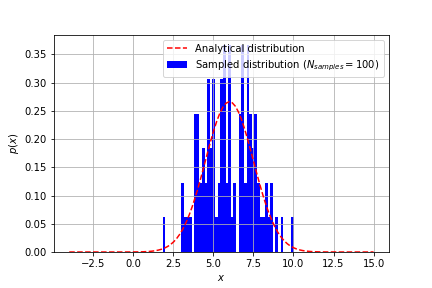
\includegraphics[width=\textwidth]{Q1a_fig1.png}
         \caption{$N_{samples} = 100$.}
     \end{subfigure}
     \hfill
     \begin{subfigure}[b]{0.3\textwidth}
         \centering
         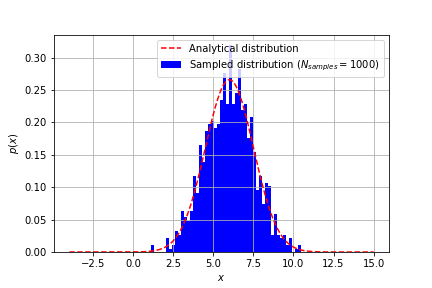
\includegraphics[width=\textwidth]{Q1a_fig2.png}
         \caption{$N_{samples} = 1000$.}
     \end{subfigure}
     \hfill
     \begin{subfigure}[b]{0.3\textwidth}
         \centering
         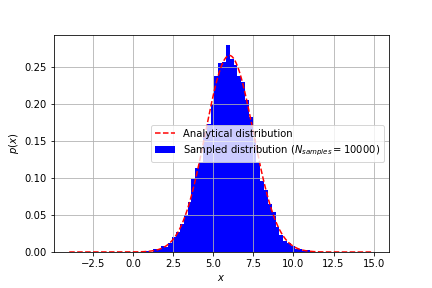
\includegraphics[width=\textwidth]{Q1a_fig3.png}
         \caption{$N_{samples} = 10 000$.}
     \end{subfigure}
        \caption{The analytical and empirical distributions of $p(x) = \mathcal{N}(6, 1.5^2)$, where the empirical distribution is demonstrated in a), b) and c) as a function of the number of samples.}
        \label{fig:Q1a_1}
\end{figure}

\subsection{The CDF of $p(x)$}

The CDF of a probability distribution is a representation of the integral
\begin{equation}
    F_x(X) = \int_{-\infty}^{X}p(x)dx = P(x \leq X),
\end{equation}
where $F_x(X)$ is the CDF. The CDF of a function is bounded $0 \leq F_x(X) \leq 1$ as probability distribution is valid if $p(x)\geq 0$ for the domain of the distribution and the integral $\int_x p(x)dx$ is required to integrate to 1. Thus, the CDF is strictly positive and is bounded $0 \leq F_x(X) \leq 1$. In figure \ref{fig:Q1a_2}, the CDF of $p(x)$ is shown.
\begin{figure}
    \centering
    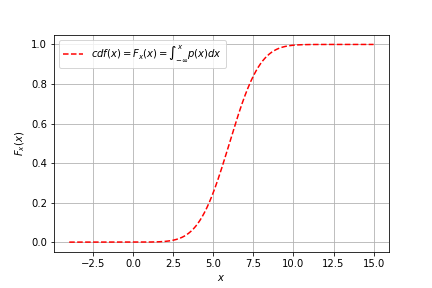
\includegraphics[scale=0.5]{Q1a_fig4.png}
    \caption{The CDF of $p(x)$.}
    \label{fig:Q1a_2}
\end{figure}

\subsection{Analytical probabilities versus Monte Carlo estimates}

In this portion of the assignment we are required to find the probability that $4 \leq x \leq 5$ using a \texttt{Python scipy.stats} method and through Monte Carlo integration. Using the definition of a CDF, we can represent the probability range of interest as
\begin{equation}\label{eq:p_4_x_5}
\begin{aligned}[b]
P_x(4 \leq x \leq 5) &= \int_{4}^{5} p(x) dx \\
&= \int_{-\infty}^{5} p(x)dx - \int_{-\infty}^{4} p(x) dx \\
\text{where the CDF of } p(x) &\text{ is defined as: } P(x \leq X) = F_x(X) = \int_{-\infty}^{X}p(x)dx \\
&= F_x(5) - F_x(4). \\
\end{aligned}
\end{equation}

Equation \eqref{eq:p_4_x_5} can be used to calculate $P_x(4 \leq x \leq 5)$ if the CDF of $p(x)$ is known. If we assume that the CDF of $p(x)$ is not known or difficult to obtain analytically, then we can turn to Monte Carlo integration. Monte Carlo integration a Monte Carlo method to numerically compute a definite integral. The definite integral of interest is
\begin{equation}
    \int_{-\infty}^{\infty} p(x)f(x)dx,
\end{equation}

which can be approximated as
\begin{equation}\label{eq:MonteCarlo}
\int_{-\infty}^{\infty}p(x)f(x)dx = \lim_{n \rightarrow \infty} \frac{1}{N} \sum_{i=1}^{N} f(x_i),
\end{equation}
where $x_i \sim p(x)$. Thus, we no longer require the CDF of $p(x)$ and simply require samples from $p(x)$ to estimate the definite integral. The definite integral of interest can also be written as the expectation
\begin{equation}
    \int_{-\infty}^{\infty}f(x)p(x)dx = \mathbb{E}_{x\sim p(x)}\{ f(x) \},
\end{equation}
which is referred to as the expectation of a function of a random variable.

To numerically determine $P(4 \leq x \leq 5)$, two indicator functions are introduced
\begin{equation}
f_4(x) = I(x; -\infty, 4) = \begin{cases} 
1 & \text{if } x \leq 5, \\
0 & \text{otherwise,}
\end{cases}
\end{equation}
where $I(x; -\infty, 4)$ is the indicator function. Additionally, let 

\begin{equation}
f_5(x) = I(x; -\infty, 5) = \begin{cases} 
1 & \text{if } x \leq 5, \\
0 & \text{otherwise.}
\end{cases}
\end{equation}

Thus, we can approximate $P(4 \leq x \leq 5)$ through
\begin{equation}
\begin{aligned}[b]
P(4 \leq x \leq 5) &= \mathbb{E}_{x\sim p(x)} \{f_5(x)\} - \mathbb{E}_{x\sim p(x)} \{f_4(x)\} \\
&= \frac{1}{N} \left( \sum_{n=1}^{N}f_5(x_n) - \sum_{n=1}^{N}f_4(x_n) \right),
\end{aligned}
\end{equation}
where $x_n \sim p(x)$. The question now becomes: \emph{why do the two indicator functions $f_4(x)$ and $f_5(x)$ work?} We know as a prior that the probability $P(4 \leq x \leq 5)$ can be decomposed into a combination of two definite integrals with an integral upper limit of $x = 5$ and $x= 4$ respectively, as shown in Equation \eqref{eq:p_4_x_5}. To approximate the two integrals, Monte Carlo integration is used and we need to ensure that samples from $p(x)$ are 'active' in each integral up to the upper integration bounds. This is equivalent to setting $p(x)$ to zero at any point above the bounds. To visualise the effect of $f_4(x)$ and $f_5(x)$ on the analytical distribution, please refer to Figure \ref{fig:Q1a_3}.
\begin{figure}
    \centering
    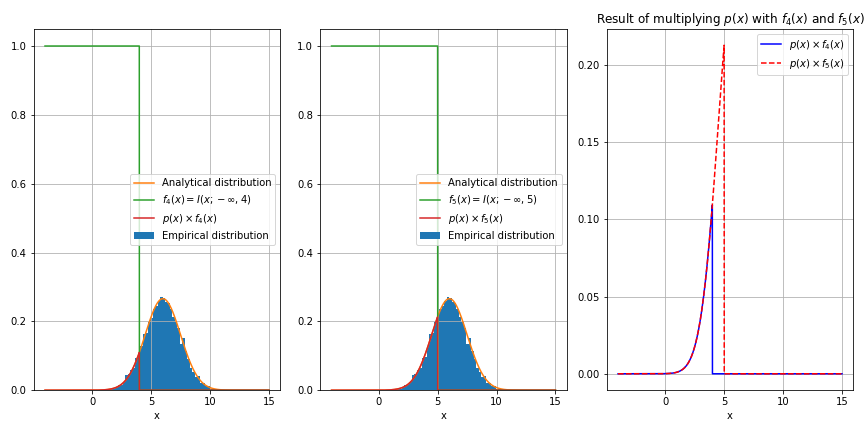
\includegraphics[scale=0.5]{Q1a_fig5.png}
    \caption{A visualisation of the indicator functions and $p(x)$, and the result of the multiplication of $f_4(x)$ and $f_5(x)$ with $p(x)$.}
    \label{fig:Q1a_3}
\end{figure}

\begin{table}[!htb]
\centering
\caption{The calculation of $P(4 \leq x \leq 5)$ by using the CDF of $p(x)$ and Monte Carlo integration.}
\label{tab:probability_calculation}
\begin{tabular}{@{}cc@{}}
\toprule
Estimation method & $P(4 \leq x \leq 5)$ \\ \midrule
CDF calculation & 0.161281 \\
Monte Carlo integration & 0.161285 \\ \bottomrule
\end{tabular}
\end{table}

In Table \ref{tab:probability_calculation} the results of the two probability calculation methods are shown. Figure \ref{fig:Q1a_4} shows the mean and variance over the Monte Carlo estimate of $P(4 \leq x \leq 5)$ as a function of the number of samples. From  Figure \ref{fig:Q1a_4}a) is clear that more samples ensures that there is less variation in the estimate, and this is also backed up by Figure \ref{fig:Q1a_4}b) which shows the estimation error between the two methods as a function of the number of samples.

\begin{figure}[!htb]
     \centering
     \begin{subfigure}[b]{0.45\textwidth}
         \centering
         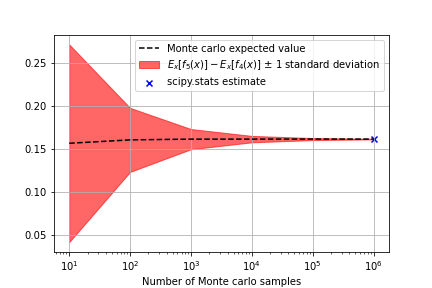
\includegraphics[width=\textwidth]{Q1a_fig6.png}
         \caption{Monte Carlo estimate versus samples.}
     \end{subfigure}
     \hfill
     \begin{subfigure}[b]{0.45\textwidth}
         \centering
         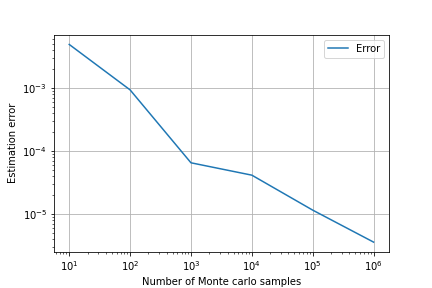
\includegraphics[width=\textwidth]{Q1a_fig7.png}
         \caption{Monte Carlo estimation error.}
     \end{subfigure}
        \caption{The expected value of the Monte Carlo estimate of $P_x(4 \leq x \leq 5)$ and the estimation error as a function of the number of samples. In a) we see that the variance around the estimate decreases with sample number. In b) we see an increase in the accuracy of the estimate of $P_x(4 \leq x \leq 5)$ as the number of samples increase.}
        \label{fig:Q1a_4}
\end{figure}

\subsubsection{Percentiles}

The CDF is a useful tool to evaluate the probability $P(x \leq X)$, and if the CDF can be inverted, then the inverse CDF serves as a useful tool to return values of the random variable $x$ that correspond to a given probability. These probability values are referred to as percentiles as the value captures a certain probability $P(x \leq X)$, and the CDF is bounded by $F_x(X) \in [0, 1]$, thus we can express the values as percentages. We can determine the $7^{th}$ percentile of x using the quantile function or by using Monte Carlo integration. In Table \ref{tab:percentile_calculation}, the results of the two methods are shown and in Figure \ref{fig:Q1a_5} the relationship between the percentile and the CDF of $p(x)$ is shown. Figure \ref{fig:Q1a_6} shows the Monte Carlo estimate as a function of the number of samples. From Figures \ref{fig:Q1a_6}a) and Figures \ref{fig:Q1a_6}b) it is clear that the accuracy of the estimate tends towards the quantile function solution if a large number of samples is used, and the variation in the estimate is also reduced.
\begin{table}[!htb]
\centering
\caption{The calculation of the $7^{th}$ percentile of $x$ by using the quantile function of $p(x)$ and Monte Carlo integration.}
\label{tab:percentile_calculation}
\begin{tabular}{@{}cc@{}}
\toprule
Estimation method & $7^{th}$ percentile \\ \midrule
quantile calculation & 3.786313 \\
Monte Carlo integration & 3.786350 \\ \bottomrule
\end{tabular}
\end{table}
\begin{figure}
    \centering
    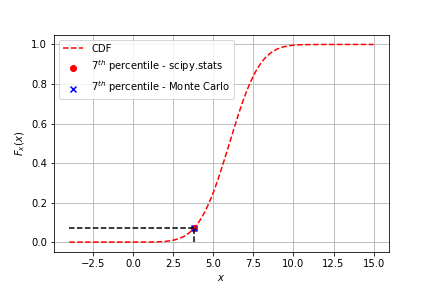
\includegraphics[scale=0.5]{Q1a_fig8.png}
    \caption{The CDF of $p(x)$ and the $7^{th}$ percentile thereof. Notice how the \texttt{scipy.stats} estimate and the Monte Carlo estimate are very close.}
    \label{fig:Q1a_5}
\end{figure}

\begin{figure}[!htb]
     \centering
     \begin{subfigure}[b]{0.45\textwidth}
         \centering
         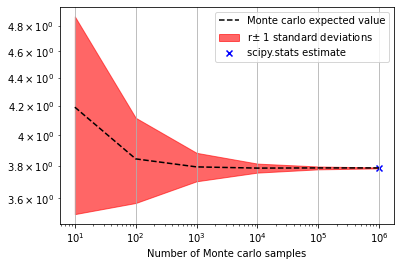
\includegraphics[width=\textwidth]{Q1a_fig9.png}
         \caption{Monte Carlo estimate versus samples.}
     \end{subfigure}
     \hfill
     \begin{subfigure}[b]{0.45\textwidth}
         \centering
         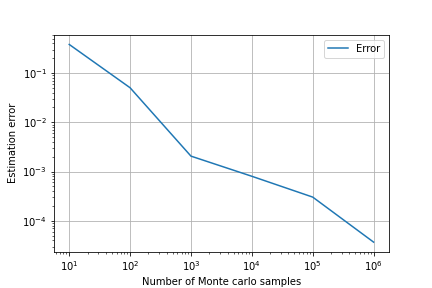
\includegraphics[width=\textwidth]{Q1a_fig10.png}
         \caption{Estimation error.}
     \end{subfigure}
        \caption{The expected value of the Monte Carlo estimate of the $7^{th}$ percentile and the estimation error as a function of the number of samples. In a) we see that the variance around the estimate decreases with sample number. In b) we see an increase in the accuracy of the estimate of  $7^{th}$ percentile as the number of samples increase.}
        \label{fig:Q1a_6}
\end{figure}

\subsubsection{Numerical quadrature vs Monte-Carlo integration}
The function within the expectation $\mathbb{E}\{ f(x) \}$ is not only limited to simple functions, but can also be applied to complex functions. Consider the following function form
\begin{equation}\label{eq:Q1_complex_function}
    f(x) = \vert e^x \cdot \cos \left( x^2 \right) \vert,
\end{equation}
where $\vert \cdot \vert$ is the absolute value function. We can determine the definite integral that the expectation represents with two methods, namely \emph{i)} numerical quadrature and \emph{ii)} Monte Carlo integration using Equation \eqref{eq:MonteCarlo}. In table \ref{tab:complex_expectations} the results from the two methods are given. As was shown for the previous Monte Carlo integration sections, Figure \ref{fig:Q1a_6} was developed to show the sensitivity of the Monte Carlo estimate of the expectation of Equation \eqref{eq:Q1_complex_function}. It is clear that the number of samples is important to this expectation, as if the number of samples is too low both the estimate variance and the estimation error is high.
\begin{table}[!htb]
\centering
\caption{The calculation of $\mathbb{E}\{ \vert e^x \cdot \cos \left( x^2 \right) \vert\}$, using numerical quadrature and Monte Carlo integration.}
\label{tab:complex_expectations}
\begin{tabular}{@{}cc@{}}
\toprule
Estimation method & $\mathbb{E}\{ \vert e^x \cdot \cos \left( x^2 \right) \vert\}$ \\ \midrule
Numerical quadrature & 791.094335 \\
Monte Carlo integration & 791.683632 \\ \bottomrule
\end{tabular}
\end{table}

\begin{figure}[!htb]
     \centering
     \begin{subfigure}[b]{0.45\textwidth}
         \centering
         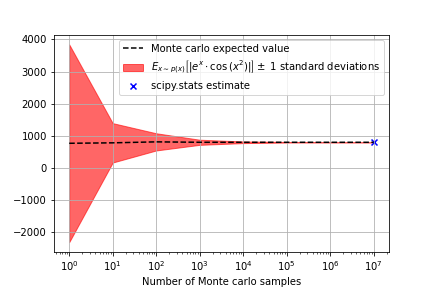
\includegraphics[width=\textwidth]{Q1a_fig11.png}
         \caption{Monte carlo estimate versus samples.}
     \end{subfigure}
     \hfill
     \begin{subfigure}[b]{0.45\textwidth}
         \centering
         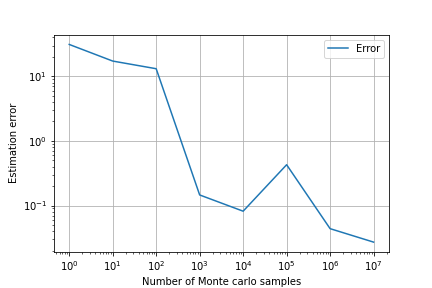
\includegraphics[width=\textwidth]{Q1a_fig12.png}
         \caption{Estimation error.}
     \end{subfigure}
        \caption{The expected value of the Monte Carlo estimate of $\mathbb{E}_{x\sim p(x)}\{\vert e^x \cdot \cos \left( x^2 \right) \vert \}$ and the estimation error as a function of the number of samples. In a) we see that the variance around the estimate decreases with sample number. In b) we see an increase in the accuracy of the estimate as the number of samples increase.}
        \label{fig:Q1a_6}
\end{figure}

\subsubsection{Log-likelihood calculations}

Given some data $\mathbf{x}$, we can evaluate the likelihood of observing this data under $p(x)$. The data of interest in this case is
\begin{equation}\label{eq:Q1a_data}
\mathbf{x} = 
\begin{bmatrix}
 4 & 5 & 6 & 7 \\
\end{bmatrix}^T.
\end{equation}
The likelihood of $\mathbf{x}$ is given as
\begin{equation}
    p(\mathbf{x}) = p(x_0, \cdots, x_N),
\end{equation}
where, if we assume that the data in $\mathbf{x}$ is independently and  identically distributed (\emph{i.i.d}), the likelihood of $\mathbf{x}$ can be written as
\begin{equation}
    p(\mathbf{x}) = \prod_{n=1}^{N}p(x_n).
\end{equation}

However, the log of $p(x)$ can be used to not only simplify the computation, but it can also avoid any numerical underflow or overflow issues. This can occur if one of the samples in $\mathbf{x}$ has a numerically small likelihood or if the variance of the distribution tends towards zero. The log-likelihood can be given as
 \begin{equation}\label{eq:Q1_log_likelihood}
 \begin{aligned}[b]
 p(\mathbf{x}) &= \prod_{n=1}^{N} p(x_n) \\
 &= \prod_{n=1}^{N}\mathcal{N}(x_n \vert \mu, \sigma^2) \\
 &= \prod_{n=1}^{N}\frac{1}{\sqrt{2\cdot\pi \sigma^2}}\exp{-\frac{1}{2\sigma^2} \left( x_n - \mu)\right)^2} \\
 \log p(\mathbf{x}) &= \sum_{n=1}^{N} \left(-\frac{1}{2} \log(2\cdot\pi) - \frac{1}{2}\log(\sigma^2) - \frac{1}{2\sigma^2} \cdot (x_n - \mu)^2 \right) \\
\mathcal{LL}(\mu, \sigma) &= -\frac{N}{2} \log(2\cdot\pi) - \frac{N}{2}\log(\sigma^2) - \frac{1}{2\sigma^2} \sum_{n=1}^{N} (x_n - \mu)^2,
 \end{aligned}
 \end{equation}
 where $\mathcal{LL}(\mu, \sigma)$ is the log-likelihood function. For the data given in Equation \eqref{eq:Q1a_data}, the log-likelihood is equal to $ \log p(\mathbf{x}) = -6.630948$.
 
 \subsection{Part B: Maximum likelihood estimates}
 
 In Figure \ref{fig:Q1b_1}, a set of samples is given from a generative distribution $p(x)$, and the objective is to use maximum likelihood estimation to model this generative distribution. The formulation here follows the model form given in Equation \eqref{eq:Model1}, and the log-likelihood function shown in Equation \eqref{eq:Q1_log_likelihood} will be used as an estimator to determine the optimal model parameters.
 \begin{figure}
     \centering
     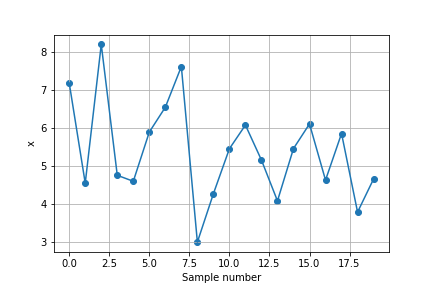
\includegraphics[scale=0.5]{Q1b_fig1.png}
     \caption{The available training data used for performing maximum likelihood estimation for the model given in Equation \eqref{eq:Model1}.}
     \label{fig:Q1b_1}
 \end{figure}

For this investigation, the following methods will be used to determine the optimal parameters:
\begin{itemize}
    \item Exhaustive grid search over the model parameters.
    \item A closed form solution will be derived and used.
    \item In-built \texttt{Python} methods.
    \item Numerical optimisation methods.
\end{itemize}

For this investigation, we need to derive the closed form solution to the maximum likelihood estimator. This can be achieved by deriving Equation \eqref{eq:Q1_log_likelihood} with respect to the model parameters $\mu$ and $\sigma$, setting the derivative to zero and re-organising the equation to obtain an estimator for the parameters. If we complete this process for $\mu$: 
\begin{equation}
\begin{aligned}
\frac{d\mathcal{LL}}{d\mu} &= -\frac{2}{2\sigma^2} \sum_{n=1}^{N} \left(x_n - \mu\right) \cdot 1\\
0 &= \sum_{n=1}^{N}\left(x_n - \mu\right) \\
\hat{\mu} &= \frac{1}{N} \sum_{n=1}^{N} x_n.
\end{aligned}
\end{equation}

If we complete this process for $\sigma$:
\begin{equation}
\begin{aligned}
\frac{d\mathcal{LL}}{d\sigma} &= -\frac{N}{2}\cdot\frac{2\sigma}{\sigma^2} -\frac{-2}{2\sigma^3} \sum_{n=1}^{N} \left(x_n - \mu\right)^2 \\
0 &=  -N + \frac{1}{\sigma^2} \sum_{n=1}^{N} \left(x_n - \mu\right)^2 \\
\sigma^2 &= \frac{1}{N} \sum_{n=1}^{N} \left(x_n - \mu\right)^2 \\
\hat{\sigma} &= \sqrt{\frac{1}{N} \sum_{n=1}^{N} \left(x_n - \mu\right)^2}.
\end{aligned}
\end{equation}
Thus, we can solve for the maximum likelihood estimates of $\mu$ and $\sigma$. In Table \ref{tab:Q2_table1}, the optimal parameters for the different methods are shown. It is clear that each method returns very similar parameters, and only the grid-search parameters are noticeably different. However this difference is only in the second decimal place.
\begin{table}[!htb]
\centering
\caption{The optimal model parameters and model log-likelihood for different parameter estimation methods.}
\label{tab:Q1b_table}
\begin{tabular}{@{}cccc@{}}
\toprule
Solution method & $\hat{\mu}$ & $\hat{\sigma}$ (biased) & model log-likelihood \\ \midrule
Grid-based & 5.3768843 & 1.285427 & -33.411642 \\
Closed-form & 5.390712 & 1.286063 & -33.410480 \\
In-built method (\texttt{scipy.stats}) & 5.390712 & 1.286063 & -33.410480 \\
Numerical optimisation & 5.390712 & 1.286063 & -33.410480 \\ \bottomrule
\end{tabular}
\end{table}

If Figure \ref{fig:Q1b_2}a) the likelihood function over the parameters $\mu$ and $\sigma$ is shown. The optimal parameters from the various methods are superimposed on the figure. It is clear that the optimal parameters are highly localised. In Figure \ref{fig:Q1b_2}b) the analytical distribution for the different methods are superimposed over the samples. It is clear that all of the methods return similar parameters. 

\begin{figure}[!htb]
     \centering
     \begin{subfigure}[b]{0.45\textwidth}
         \centering
         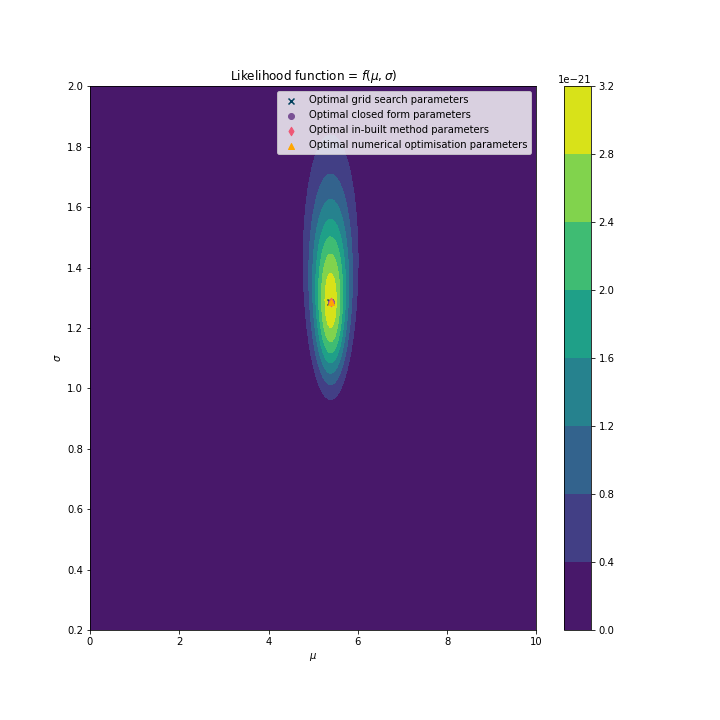
\includegraphics[width=\textwidth]{Q1b_fig2.png}
         \caption{Likelihood function.}
     \end{subfigure}
     \hfill
     \begin{subfigure}[b]{0.45\textwidth}
         \centering
         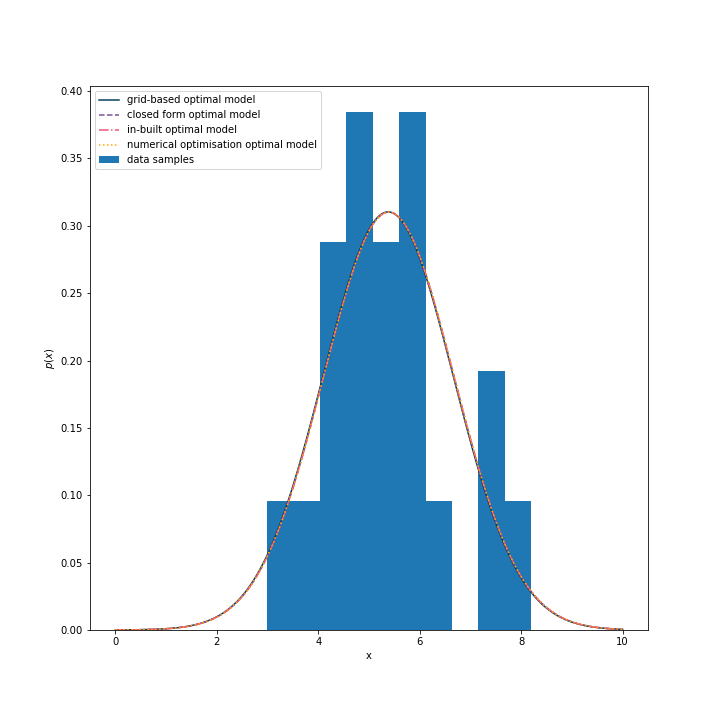
\includegraphics[width=\textwidth]{Q1b_fig3.png}
         \caption{Model visualisation.}
     \end{subfigure}
        \caption{The likelihood function over the model parameters $\mu$ and $\sigma$ for the methods of interest. In a) the optimal parameters are superimposed over the likelihood function, and in b) the optimal models are superimposed over the data samples.}
        \label{fig:Q1b_2}
\end{figure}

Finally, it is also possible to investigate the confidence interval over $\mu$. As the model variance $\sigma^2$ is unknown, the confidence interval calculation is given as
\begin{equation}
    \mathcal{T}_{\alpha/2, N-1} \leq \mu \leq \mathcal{T}_{1-\alpha/2, N-1},
\end{equation}
where $\mathcal{T}_{\nu, dof}$ is the $(\nu\cdot 100)^{th}$ percentile of a Student t distribution defined as $\text{st}_{dof}\left(\hat{\mu}, \hat{\sigma}^2/N \right)$. Note that $\tilde{\sigma}^2$ is the unbiased estimate of the maximum likelihood estimate $\hat{\sigma}$, given as 
\begin{equation}
    \tilde{\sigma} = \sqrt{\frac{1}{N-1} \sum_{n=1}^{N} \left(x_n - \mu\right)^2}.
\end{equation}

When using the maximum likelihood estimates for $\mu$ and $\sigma$, as detailed in Table \ref{tab:Q1b_table}, the unbiased estimate of $\sigma$ is $\tilde{\sigma} = 1.319473$. The resulting confidence interval is
\begin{equation}
    4.773179 \leq \mu \leq 6.008244.
\end{equation}

In Figure \ref{fig:Q1b_3}, the confidence interval is visualised over the data samples and the Student t distribution with $dof=19$, a location parameter equation to $\hat{\mu}$ and a scale parameter equation to $\tilde{\sigma}/N$. 
 \begin{figure}
     \centering
     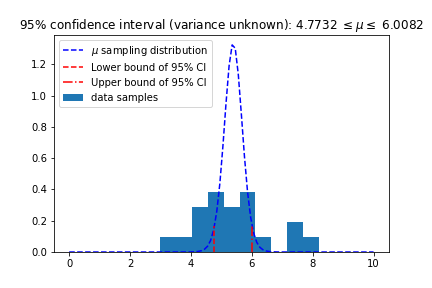
\includegraphics[scale=0.6]{Q1b_fig4.png}
     \caption{The 95$\%$ confidence interval on $\mu$ for a model where the variance is also a function of the data.}
     \label{fig:Q1b_3}
 \end{figure}
 
 \subsection{Part C: Sampling distributions}
 
 \subsubsection{Empirical and analytical sampling distributions}
 Let us assume that the true model parameters are $\mu=6$ and $\sigma = 1.5$. As the maximum likelihood estimate is a function of the data,  we can define a probability distribution over any random sample-based estimate. This occurs as the estimate is calculated using a subset of the true population and thus the estimator is also a random variable. The distribution over the estimate is referred to as the sampling distribution. If the estimate is the mean $\mu$ and it is assumed that $\sigma$ is known, we expect the analytical form of the sampling distribution to be $p_{\mu}(x) = \mathcal{N}(\mu, \sigma^2/N)$, where $N$ is the number of samples used to estimate $\hat{\mu}$.

To compare the sampling distribution to the empirical sampling distribution, we will will iterative repeat the following process:
\begin{enumerate}
    \item Draw 20 samples from $p(x) = \mathcal{N}(6, 1.5^2)$.
    \item Calculate the maximum likelihood estimate $\hat{\mu}$.
    \item Store estimate and repeat the steps 10 000 times.
\end{enumerate}
 
 If Figure \ref{fig:Q1c_1} the analytical and empirical sampling distribution for $\mu$ is shown. It is clear that the two distributions are highly similar. As the number of samples increases, we would expect that the empirical distribution clearly tend towards the analytical distribution.
 \begin{figure}[!htb]
     \centering
     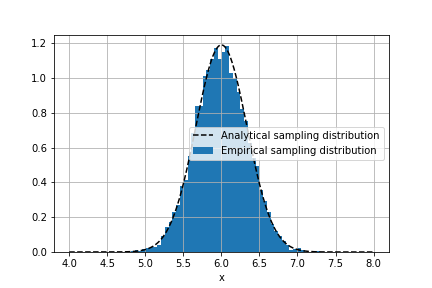
\includegraphics[scale=0.6]{Q1c_fig1.png}
     \caption{The empirical and analytical sampling distributions for the model presented in Equation \eqref{eq:Model1} with $\mu=6$ and $\sigma=1.5$. The empirical distribution was generated by drawing 20 samples from the true model $x\sim \mathbb{N}(6, 1.5^2)$ and then calculating the maximum likelihood estimate for $\hat{\mu}$ repeatedly.}
     \label{fig:Q1c_1}
 \end{figure}
 
 \subsubsection{Estimator bias}
 Although estimators can be derived analytically to maximise a log-likelihood function, an estimator may be biased by the number of samples used, as it is a function of the sampled data. The hope is that the estimator, which we expect to vary as we re-sample the data, be equal or approximately equal to the true population estimator. If this is the case, then we would expect that the bias of an estimator $\theta$
 \begin{equation}
     bias(\theta) = \theta - \mathbb{E}\{ \hat{\theta} \} = 0,
 \end{equation}
 where $\mathbb{E}\{ \hat{\theta} \}$ estimates the mean of the sampling distribution over $\hat{\theta}$. Naturally, this may not apply to all estimators, and for Gaussian distributions it is well known that the variance estimator is biased ($\text{bias}(\sigma) \ne 0$) and it can be corrected with the Bessel's correction factor. The biased variance estimator $\hat{\mu}$ is unbiased through 
 \begin{equation}
    \tilde{\sigma} = \frac{N}{N - 1} \hat{\sigma},
 \end{equation}
 where $\tilde{\sigma}$ is the unbiased variance estimator and $\frac{N}{N - 1}$ is the Bessel correction factor. We can derive this factor analytically, but we can also demonstrate the bias through Monte Carlo estimation of $\mathbb{E}\{\hat{\sigma}\}$. For this example, let estimator one be
 \begin{equation}
    \sigma_1 = \frac{1}{N}\sum_{n=1}^{N} \left( x_n - \hat{\mu} \right)^2,
\end{equation}
and let estimator two be
\begin{equation}
    \sigma_2 = \frac{1}{N - 1}\sum_{n=1}^{N} \left( x_n - \hat{\mu} \right)^2.
\end{equation}
 
 In Figure \ref{fig:Q1c_2}, the bias of the and the variance of this bias as a function of the number of samples used to perform Monte Carlo integration is shown. Figure \ref{fig:Q1c_2}a) has a clear bias expectation offset, while Figure \ref{fig:Q1c_2}b) has a bias expectation term equal to 0. Figure \ref{fig:Q1c_2} clearly shows that estimator two is the unbiased estimator for $\sigma_2$. However, an unbiased estimator is not optimal when maximising the log-likelihood function, and thus the decision to bias or unbias the estimator depends on how the model is applied. If the model is used to provide intuition or interpretation to some data, then the unbiased estimate is preferred. However, in cases where the model is used to evaluate whether new data is from the observed data, then increasing unbiasing the variance could potentially cause problems. The variance around the bias was determined by repeating the bias estimation process numerous times. This variance is present as the bias is a random variable due to the dependence on $\mathbb{E}\left(\hat{\sigma}_{i}\right)$, where $i = 1, 2$, which is a function of the data.
 \begin{figure}[!htb]
     \centering
     \begin{subfigure}[b]{0.45\textwidth}
         \centering
         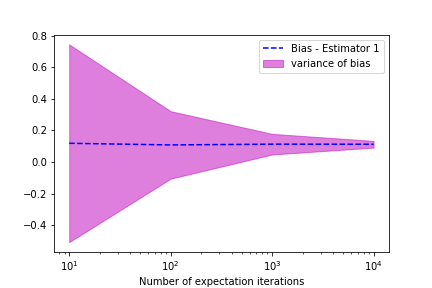
\includegraphics[width=\textwidth]{Q1c_fig2.png}
         \caption{Estimator one - $\hat{\sigma}_1^2$.}
     \end{subfigure}
     \hfill
     \begin{subfigure}[b]{0.45\textwidth}
         \centering
         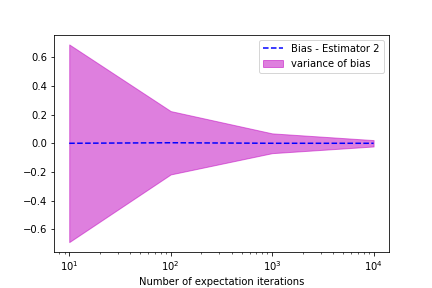
\includegraphics[width=\textwidth]{Q1c_fig3.png}
         \caption{Estimator two - $\hat{\sigma}_2^2$.}
     \end{subfigure}
        \caption{The bias of to estimators for the variance as a function of the number of expectation iterations. Notice that a) has a bias offset, while b) does not.}
        \label{fig:Q1c_2}
\end{figure}

\clearpage

\section{Question 2}

\subsection{Problem formulation}
Consider the following regression model

\begin{equation}
y_n = f(x_n) + \epsilon_n,
\end{equation}
where $\epsilon_n \sim \mathcal{N}(0, \sigma^2)$ and
\begin{equation}
f(x) = \omega_0 + \omega_1 \cdot x + \omega_2 \cdot x^2 + \cdots +  + \omega_K \cdot x^K,
\end{equation}
is a $K^{th}$ order polynomial function. The objective is to investigate regression models and how maximum likelihood estimation is used to determine the optimal model parameters and what considerations one must be aware of when fitting regression models to data. 

\begin{table}[!htb]
\centering
\caption{Parameters of the four second order polynomial models.}
\label{tab:Q2_table1}
\begin{tabular}{cccc}
\hline
Model & $\omega_0$ & $\omega_1$ & $\omega_2$ \\ \hline
Model 1 & 1 & 0 & 0 \\
Model 2 & 1 & 1 & 1 \\
Model 3 & 1 & 2 & 3 \\
Model 4 & 1 & 1 & 1 \\ \hline
\end{tabular}
\end{table}
 If Table \ref{tab:Q2_table1} different models are given and in Figure \ref{fig:Q2a_1}a) the available training data  is superimposed over the different models. To distinguish between the fit of different models, the absolute difference between the training data and the model evaluation at the $x$ points of the training data. It is clear from Figure \ref{fig:Q2a_1}b) that model two is a poor fit to the data, as it has a large error. The best candidate model, of the four models detailed in Table \ref{tab:Q2_table1}, appears to be model one as it has an error that is consistently low. 
\begin{figure}[!htb]
     \centering
     \begin{subfigure}[b]{0.45\textwidth}
         \centering
         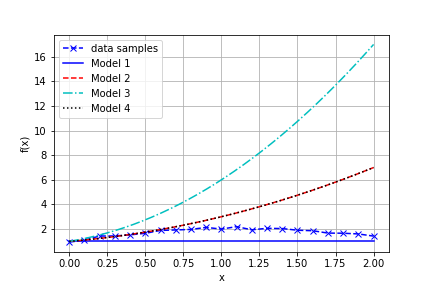
\includegraphics[width=\textwidth]{Q2a_fig1.png}
         \caption{Model visualisation.}
     \end{subfigure}
     \hfill
     \begin{subfigure}[b]{0.45\textwidth}
         \centering
         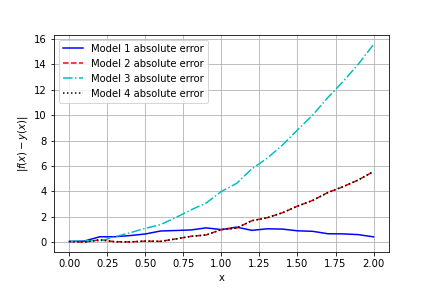
\includegraphics[width=\textwidth]{Q2a_fig2.png}
         \caption{Absolute error visualisation.}
     \end{subfigure}
        \caption{The four second order polynomials superimposed on the data samples and the absolute sample error. In a) the four models are visualised and in b) the  absolute error between the available data samples and the various model function values $f(x_n)$ is shown.}
        \label{fig:Q2a_1}
\end{figure}

\subsection{Formulating the maximum likelihood estimation problem}

The maximum likelihood problem can be formulated as follows: First it assumed that there is access to a dataset $\mathcal{D} = \{ \mathbf{X}, \mathbf{t}\}$, where $\mathbf{X} = [x_1, \cdots, x_N]^T$ and $\mathbf{t} = [t_1, \cdots, t_N]^T$, $\mathbf{X} \in \mathbb{R}^{N \times 1}$, $\mathbf{t} \in \mathbb{R}^{N \times 1}$. The following homoscedastic model formulation is then assumed for the data
\begin{equation}
t_n = f(x_n) + \epsilon_n,
\end{equation}
where $\epsilon_n \sim \mathcal{N}(0, \sigma^2)$ and
\begin{equation}
f(x) = \omega_0 + \omega_1 \cdot x + \omega_2 \cdot x^2 + \cdots +  + \omega_K \cdot x^K,
\end{equation}
is a $K^{th}$ order polynomial function. We can reformulate $f(x)$ as
\begin{equation}
f(x) = \boldsymbol\omega^T \boldsymbol\phi(x),
\end{equation}
where $\boldsymbol\omega \in \mathbb{R}^{K + 1}$ is a column vector and $\boldsymbol\phi(x)$ is a basis column vector in the form
\begin{equation}
\boldsymbol\phi(x_n) = [\phi_{n}^{(0)}, \phi_{n}^{(1)}, \cdots, \phi_{n}^{(K)}]= [x^{0}, x^{1}, \cdots, x^{K}]^T,
\end{equation}
where $\boldsymbol\phi(\cdot) \in \mathbb{R}^{K + 1}$ and $\phi_{n}^{(i)}$ refers to the $i^{th}$ index for the $n^{th}$ input $\phi_{n}^{(i)} = \boldsymbol\phi(x_n)[i]$. As the noise is an additive Gaussian distribution, the addition of $f(x)$ to $\epsilon$ gives a mean-shifted conditional Gaussian distribution
\begin{equation}
p(t\vert x) = \mathcal{N}(t \vert f(x), \sigma^2).
\end{equation}

In order to derive an estimator for this model, we assume that the samples in $\mathcal{D}$ satisfy the \emph{i.i.d} assumption. As such, we can calculate the conditional likelihood function $p(T \vert X)$ may be written as
\begin{equation}
p(T \vert X) = \prod_{n=1}^{N} p(t_n \vert x_n).
\end{equation}

However, to avoid numerical underflow issues, and to both improve and simplify derivative computations, we typically take the logarithm of the likelihood function, which gives
\begin{equation}\label{eq:Q2_log_likelihood_function}
\begin{aligned}[b]
\log p(T \vert X) &= \sum_{n=1}^{N} p(t_n \vert x_n) \\
\mathcal{L}(\boldsymbol\omega, \sigma^2) &= \sum_{n=1}^{N} \left( -\frac{1}{2}\log \left( 2\pi \right) -\frac{1}{2}\log \left( \sigma^2 \right) - \frac{1}{2\sigma^2} \left[ t_n - f(x_n)\right] ^2 \right) \\
&= -\frac{N}{2}\log \left( 2\pi \right) - \frac{N}{2}\log \left( \sigma^2 \right) - \frac{1}{2\sigma^2}\sum_{n=1}^{N}\left[ t_n - f(x_n)\right] ^2,
\end{aligned}
\end{equation}
where $\mathcal{L}(\mathbf{w}, \sigma^2)$ is the log-likelihood function that is to be maximised. This function gives an indication of how well $f(x)$ fits the training data in $\mathcal{D}$. To maximise this function, we can use numerous methods, such as performing a grid search or numerical optimisation, but let us proceed with an analytical procedure to deriving the estimators $g(\hat{\boldsymbol\omega})$ and $g(\hat{\sigma}^2)$. 

First, let us derive $\mathcal{L}(\boldsymbol\omega, \sigma^2)$ with respect to $\boldsymbol\omega$:
\begin{equation}\label{eq:partial_ML_regression}
\begin{aligned}[b]
0 &= \frac{d\mathcal{L}}{d\boldsymbol\omega} \\
&= \frac{d\mathcal{L}}{df} \frac{df}{d\boldsymbol\omega} \\
&= -\sum_{n=1}^{N}\frac{1}{\sigma^2} \left[ t_n - f(x_n) \right] \frac{df}{d\boldsymbol\omega}  \\
&= \sum_{n=1}^{N}\frac{1}{\sigma^2} \left[ t_n - f(x_n) \right]\boldsymbol\phi^T(x_n)\\
&= \sum_{n=1}^{N} t_n \boldsymbol\phi^T(x_n) - f(x_n) \boldsymbol\phi^T(x_n) \\
&= \sum_{n=1}^{N} t_n \boldsymbol\phi^T(x_n) - \boldsymbol\omega^t \boldsymbol\phi(x_n) \boldsymbol\phi^T(x_n) \\
&= \sum_{n=1}^{N} t_n \boldsymbol\phi^T(x_n) - \boldsymbol\omega^t \sum_{n=1}^{N} \boldsymbol\phi(x_n) \boldsymbol\phi^T(x_n),
\end{aligned}
\end{equation}
where the derivative $\frac{df}{d\boldsymbol\omega}$ can be found using Equation (69) from the The Matrix Cookbook \cite{Petersen2006TheMC}. Now, let us think about what the observed equation tells us. In the first term we are weighting  $\boldsymbol\phi^T(x_n)$ by $t_n$, and this can be easily expanded into a vector form through
\begin{equation}
\begin{bmatrix}
t_1  & t_2  & \vdots & t_N \\
\end{bmatrix}
\begin{bmatrix}
\phi_1^{(0)} & \phi_1^{(1)} & \cdots & \phi_1^{(K)} \\
\phi_2^{(0)} & \phi_2^{(1)} & \cdots & \phi_2^{(K)} \\
\vdots & \vdots & \ddots & \vdots \\
\phi_N^{(0)} & \phi_N^{(1)} & \cdots & \phi_N^{(K)} \\
\end{bmatrix}
= \mathbf{t}^T\boldsymbol\Phi,
\end{equation}
where 
\begin{equation}\label{eq:Phi_matrix}
\boldsymbol\Phi = 
\begin{bmatrix}
\phi_1^{(0)} & \phi_1^{(1)} & \cdots & \phi_1^{(K)} \\
\phi_2^{(0)} & \phi_2^{(1)} & \cdots & \phi_2^{(K)} \\
\vdots & \vdots & \ddots & \vdots \\
\phi_N^{(0)} & \phi_N^{(1)} & \cdots & \phi_N^{(K)} \\
\end{bmatrix},
\end{equation}
is the basis vector matrix such that the $n^{th}$ row of $\boldsymbol\Phi$ is equal to $\boldsymbol\phi(x_n)^T$ and $\boldsymbol\Phi \in \mathbb{R}^{N \times K + 1}$. If we inspect the shape of the resulting matrix, we have a $\mathbb{R}^{(1 \times N) \times (N \times K + 1)} = \mathbb{R}^{1 \times K + 1}$ matrix, which we would expect based on the current form of the first term, which is a sum of $t_n$ weighted row vectors.

In term two of the objective function, we see that we have a summation over $N$ of the outer product $\boldsymbol\phi(x_n) \boldsymbol\phi^T(x_n)$. Let us first expand this outer product and then think about methods to vectorise this process. The outer product $\boldsymbol\phi(x_n) \boldsymbol\phi^T(x_n)$ is equal to
\begin{equation}
\begin{aligned}[b]
\boldsymbol\phi(x_n) \boldsymbol\phi^T(x_n)
&= \begin{bmatrix}
\phi^{(0)}(x_n) \\
\phi^{(1)}(x_n) \\
\vdots \\
\phi^{(K)}(x_n)
\end{bmatrix}
\begin{bmatrix}
\phi^{(0)}(x_n) & \phi^{(1)}(x_n) & \cdots & \phi^{(K)}(x_n)
\end{bmatrix} \\
&= 
\begin{bmatrix}
\phi^{(0)}(x_n)\phi^{(0)}(x_n) & \phi^{(0)}(x_n)\phi^{(1)}(x_n) & \cdots & \phi^{(0)}(x_n)\phi^{(K)}(x_n) \\
\phi^{(1)}(x_n)\phi^{(0)}(x_n) & \phi^{(1)}(x_n)\phi^{(1)}(x_n) & \cdots & \phi^{(1)}(x_n)\phi^{(K)}(x_n) \\
\vdots & \vdots & \ddots & \vdots \\
\phi^{(K)}(x_n)\phi^{(0)}(x_n) & \phi^{(K)}(x_n)\phi^{(1)}(x_n) & \cdots & \phi^{(K)}(x_n)\phi^{(K)}(x_n) \\
\end{bmatrix}.
\end{aligned}
\end{equation}

If we sum $N$ of these outer products, we end up with $N$ matrices of size $\mathbb{R}^{K \times K}$ that are summed together. This can be vectorised as
\begin{equation}
\sum_{n=1}^N \boldsymbol\phi(x_n) \boldsymbol\phi^T(x_n) = \boldsymbol\Phi^T \boldsymbol\Phi,
\end{equation}
To demonstrate this, the form of $\boldsymbol\Phi$ given in Equation \eqref{eq:Phi_matrix} is used to obtain
\begin{equation}
\boldsymbol\Phi^T \boldsymbol\Phi = 
\begin{bmatrix}
\phi_1^{(0)} & \phi_2^{(0)} & \cdots & \phi_N^{(0)}  \\
\phi_1^{(1)} & \phi_2^{(1)} & \cdots & \phi_N^{(1)} \\
\vdots & \vdots & \ddots & \vdots \\
\phi_1^{(K)} & \phi_2^{(K)} & \cdots & \phi_N^{(K)}
\end{bmatrix}
\begin{bmatrix}
\phi_1^{(0)} & \phi_1^{(1)} & \cdots & \phi_1^{(K)} \\
\phi_2^{(0)} & \phi_2^{(1)} & \cdots & \phi_2^{(K)} \\
\vdots & \vdots & \ddots & \vdots \\
\phi_N^{(0)} & \phi_N^{(1)} & \cdots & \phi_N^{(K)} \\
\end{bmatrix},
\end{equation}
where we can see that the expansion of this matrix multiplication gives us our desired outcome. Thus, the objective function in Equation \eqref{eq:partial_ML_regression} can simplify terms to 
\begin{equation}
\begin{aligned}[b]
0 &= \mathbf{t}^T\boldsymbol\Phi  - \boldsymbol\omega^T \boldsymbol\Phi^T \boldsymbol\Phi \\
\boldsymbol\omega^T \boldsymbol\Phi^T \boldsymbol\Phi &= \mathbf{t}^T\boldsymbol\Phi,
\end{aligned}
\end{equation}
which is almost a solvable linear system of equations in the form $\mathbf{A}\mathbf{x} = \mathbf{b}$, but we need to put in just a little bit more work to solve the final system. By using the transpose, we get
\begin{equation}
\begin{aligned}
\boldsymbol\Phi^T \boldsymbol\Phi \boldsymbol\omega  &= \boldsymbol\Phi^T \mathbf{t} \\
\hat{\boldsymbol\omega}  &= \left( \boldsymbol\Phi^T \boldsymbol\Phi \right)^{-1} \boldsymbol\Phi^T \mathbf{t},
\end{aligned}
\end{equation}
which gives us an analytical equation to solve for the maximum likelihood estimate of $\boldsymbol\omega$ \cite{bishop2006}.

Finally, let us derive $\mathcal{L}(\boldsymbol\omega, \sigma^2)$ with respect to $\sigma^2$:
\begin{equation}
\begin{aligned}[b]
0 &= \frac{d\mathcal{L}}{d\sigma^2} \\
&= \sum_{n=1}^{N} \left( -\frac{1}{2\sigma^2} + \frac{1}{2(\sigma^2)^2} \right)\left[ t_n - f(x_n)\right] ^2 \\
&= \frac{1}{2\sigma^2}\sum_{n=1}^{N} \left( -1 + \frac{1}{\sigma^2} \right)\left[ t_n - f(x_n)\right] ^2 \\
&= \frac{1}{2\sigma^2}\left(-N + \frac{1}{\sigma^2}\sum_{n=1}^{N} \left[ t_n - f(x_n)\right] ^2 \right),
\end{aligned}
\end{equation}
and, after some re-arranging an estimator for $\sigma$ is obtained
\begin{equation}
\hat{\sigma} = \sqrt{\frac{1}{N}\sum_{n=1}^{N} \left[ t_n - f(x_n)\right] ^2}.
\end{equation}

Thus, to summarise, we have two estimators of interest for which we want to find roots for 
\begin{equation}
g(\hat{\boldsymbol\omega}) = \frac{d\mathcal{L}}{d\boldsymbol\omega},
\end{equation}
and 
\begin{equation}
g(\hat{\sigma}^2) = \frac{d\mathcal{L}}{d\sigma^2},
\end{equation}
from which we can obtain the roots to these estimators analytically using
\begin{equation}
\hat{\boldsymbol\omega} = \left( \boldsymbol\Phi^T \boldsymbol\Phi \right)^{-1} \boldsymbol\Phi^T \mathbf{t},
\end{equation}
and 
\begin{equation}
\hat{\sigma} = \sqrt{\frac{1}{N}\sum_{n=1}^{N} \left[ t_n - f(x_n)\right] ^2}.
\end{equation}

\subsection{Likelihood function intuition}

Before we perform maximum likelihood estimation for the regression problem, we can use the log-likelihood function given in Equation \eqref{eq:Q2_log_likelihood_function} to measure the goodness of fit of the four models given in Table \ref{tab:Q2_table1}. In Table \ref{tab:Q2_table2} the models and the resulting log-likelihood are shown.
\begin{table}[!htb]
\centering
\caption{model Log-likelihood for the observed data for the four second order polynomial models.}
\label{tab:Q2_table2}
\begin{tabular}{@{}cccccc@{}}
\toprule
Model & $\omega_0$ & $\omega_1$ & $\omega_2$ & $\sigma$ & Log-likelihood \\ \midrule
Model 1 & 1 & 0 & 0 & 1 & -7.663516 \\
Model 2 & 1 & 1 & 1 & 1 & -62.695407 \\
Model 3 & 1 & 2 & 3 & 4 & -36.829007 \\
Model 4 & 1 & 1 & 1 & 0.2 & -1543.721213 \\ \bottomrule
\end{tabular}
\end{table}
It is clear that the log-likelihood results match the previous model evaluation procedure using the absolute difference, as model one has the lowest log-likelihood. However, it is clear that model four is the worst model, which does not follow the previous observation that was made. This poor performance is attributed to the small model variance, as the variance is the only differentiating term between model two and model four. 

\subsection{Linear regression maximum likelihood estimation}
If we use maximum likelihood estimation to determine the model parameters, we can also investigate how well different model polynomial orders fit the data. In Figure \ref{fig:Q2a_2}, the optimal models are given for orders zero through nine, and in Table \ref{tab:Q2_table3} the model parameters are shown alongside the log-likelihood of the model for the given data. 
\begin{figure}
    \centering
    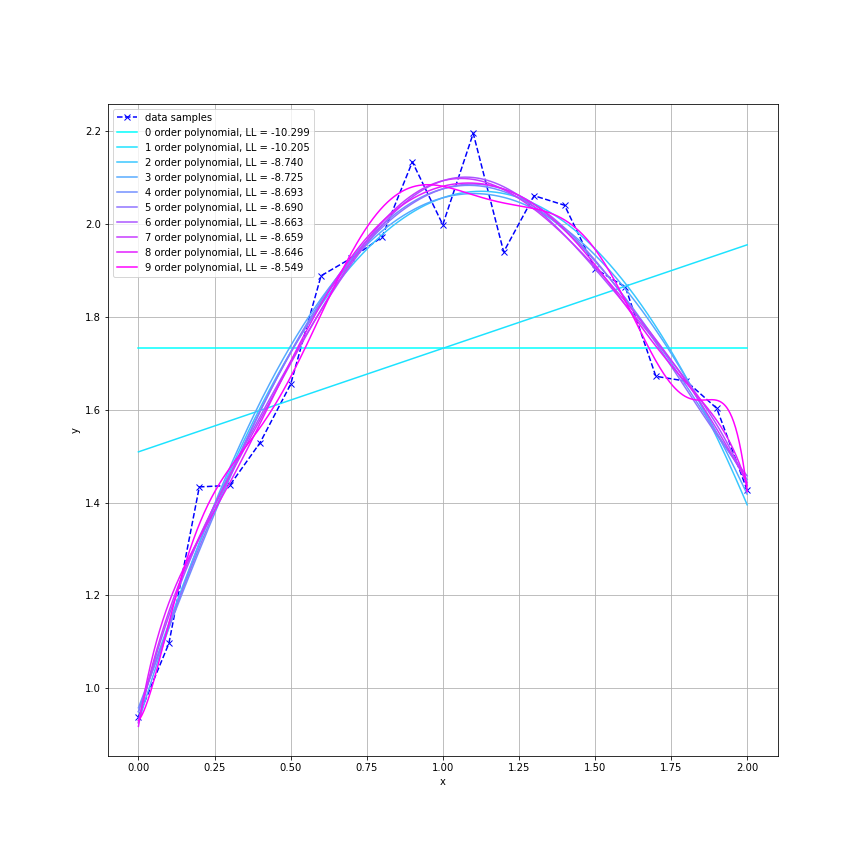
\includegraphics[scale=0.3]{Q2a_fig3.png}
    \caption{The different models with parameters from Table \ref{tab:Q2_table3} visualised over the available data samples.}
    \label{fig:Q2a_2}
\end{figure}

It is clear from Figure \ref{fig:Q2a_2} that all models of order two and above fit the available data well, and this is followed up by the model log-likelihood given in Table \ref{tab:Q2_table3}. Table \ref{tab:Q2_table3} also highlights the potential dangers of using the log-likelihood of the training data as a measure for goodness of fit, as model order two appears to be optimal, but higher model orders have better log-likelihoods. We can also observe some saturation in the results in Table \ref{tab:Q2_table3} for $\hat{\omega}_0$ and $\hat{\sigma}$ for orders two and above.
\begin{table}[!htb]
\centering
\caption{The model parameters for the maximum likelihood estimate for different sets of unknown model parameters. The order was increased linearly from $k=0$ to $k=9$.}
\label{tab:Q2_table3}
\resizebox{\textwidth}{!}{%
\begin{tabular}{@{}ccccccccccccc@{}}
\toprule
Model & $\hat{\omega}_0$ & $\hat{\omega}_1$ & $\hat{\omega}_2$ & $\hat{\omega}_3$ & $\hat{\omega}_4$ & $\hat{\omega}_5$ & $\hat{\omega}_6$ & $\hat{\omega}_7$ & $\hat{\omega}_8$ & $\hat{\omega}_9$ & $\hat{\sigma}$ & Log-likelihood \\ \midrule
Model 1 & 1.732089 &  &  &  &  &  &  &  &  &  & 0.32617 & -10.298603 \\
Model 2 & 1.509169 & 0.22292 &  &  &  &  &  &  &  &  & 0.296928 & -10.204673 \\
Model 3 & 0.94936 & 1.990735 & -0.883908 &  &  &  &  &  &  &  & 0.068606 & -8.739562 \\
Model 4 & 0.926626 & 2.146419 & -1.083332 & 0.066475 &  &  &  &  &  &  & 0.067644 & -8.725439 \\
Model 5 & 0.958109 & 1.743005 & -0.123532 & -0.691619 & 0.189523 &  &  &  &  &  & 0.065484 & -8.692988 \\
Model 6 & 0.950086 & 1.923687 & -0.817186 & 0.264042 & -0.353809 & 0.108666 &  &  &  &  & 0.065294 & -8.690085 \\
Model 7 & 0.930373 & 2.692257 & -5.20073 & 9.484886 & -9.186001 & 4.024855 & -0.652698 &  &  &  & 0.063522 & -8.662568 \\
Model 8 & 0.925207 & 3.047982 & -8.04435 & 17.925987 & -21.158875 & 12.772384 & -3.829175 & 0.453782 &  &  & 0.063308 & -8.659189 \\
Model 9 & 0.918081 & 3.960431 & -17.788745 & 56.548011 & -96.372556 & 92.554489 & -50.832193 & 14.899211 & -1.805679 &  & 0.062499 & -8.646328 \\
Model 10 & 0.930473 & 0.759279 & 25.898768 & -164.735617 & 465.12084 & -710.8877 & 626.878956 & -319.159053 & 87.160201 & -9.885095 & 0.056724 & -8.549389 \\ \bottomrule
\end{tabular}%
}
\end{table}

\subsection{Parameter confidence interval}

The $100 \cdot \gamma\%$ confidence intervals of the $k^{th}$ weight is given as
\begin{equation}
\hat{\omega}_k - t_{(1+\gamma)/2} \sqrt{\Sigma_{kk}} \leq \omega_k \leq \hat{\omega}_k + t_{(1+\gamma)/2} \sqrt{\Sigma_{kk}},
\end{equation}

where $t_{(1+\gamma)/2}$ is the $t$-statistic with $N - K - 1$ degrees of freedom. This can be re-written as
\begin{equation}
t_{(1-\gamma)/2}\left(\hat{\omega}_k, \Sigma_{kk}\right) \leq \omega_k \leq t_{(1+\gamma)/2}\left(\hat{\omega}_k, \Sigma_{kk}\right).
\end{equation}

The covariance matrix $\boldsymbol\Sigma$ is given as
\begin{equation}
\boldsymbol\Sigma = \tilde{\sigma}^2 \mathbf{A},
\end{equation}

and the matrix $\mathbf{A}$ is equal to
\begin{equation}
\mathbf{A} = \left( \boldsymbol\Phi^T\boldsymbol\Phi \right)^{-1}.
\end{equation}

It is important to note here that $\tilde{\sigma}^2$ refers to the unbiased maximum likelihood estimate of the linear regression model variance, given as 
\begin{equation}
\tilde{\sigma}^2 = \frac{N}{N - K - 1}\hat{\sigma}^2.
\end{equation}

If we calculate this confidence interval for a model order of two, we obtain 
\begin{equation}
    0.873 \leq \omega_0 \leq 1.026.
\end{equation}
Figure \ref{fig:Q2a_3} shows the upper and lower confidence interval bounds if we repeat this process for model orders zero through nine. Notice that the parameter bounds steady out for orders two and above, with the tightest bound being around order two. This suggests that the unbiased regression model variance increased, which is a potential indicator that model orders larger than two worsen the estimator performance.
\begin{figure}
    \centering
    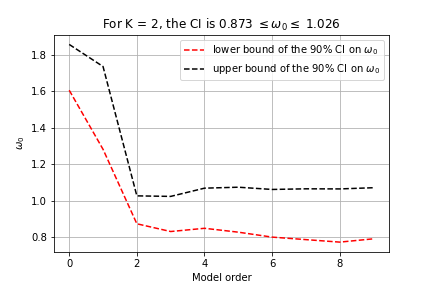
\includegraphics[scale = 0.5]{Q2a_fig4.png}
    \caption{The confidence interval around $\omega_0$ as a function of the model order. Notice how after $K=2$ the confidence interval appears to smooth out.}
    \label{fig:Q2a_3}
\end{figure}

\subsection{Model selection investigation}
Consider the following fifth order polynomial
\begin{equation}
    f(x) = 3 + 0.2 \cdot x + 1 \cdot x^2 -0.45 \cdot x^3 + 0.2 \cdot x^4 -0.1 \cdot x^5,
\end{equation}
from which we can sample data. To perform this sampling, a uniform distribution $U[-2, 3]$ is assumed over $x$, and this distribution is sampled in order to generate samples from $f(x)$. Finally, samples from $y$ are obtained through the inclusion of additive Gaussian noise $\epsilon\sim \mathbb{N}(0, 0.1^2)$. In Figure \ref{fig:Q2b_1}, an example of the polynomial samples is shown. 
\begin{figure}[!htb]
    \centering
    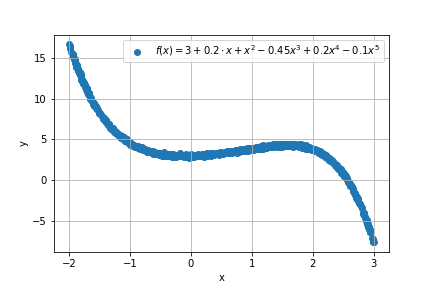
\includegraphics[scale=0.5]{Q2b_fig1.png}
    \caption{The polynomial function of interest for the model selection investigation.}
    \label{fig:Q2b_1}
\end{figure}

For this investigation, the objective is to explore how the following four model selection methods, namely \emph{i)} negative log-likelihood (NLL), \emph{ii)} Akaike information criterion (AIC), \emph{iii)} Bayesian information criterion (BIC), and \emph{iv)} mean-squared error (MSE) affect the selection of an optimal model. To further this investigation, the aforementioned selection methods will be used on the training data alone and on the test data from a $k$-fold cross validation setting. In this write-up, the standard setting will be used to refer to the former and the cross-validation setting will refer to the latter. The objective here is to investigate how the methods perform when we evaluate them on the data used to develop the model, versus if we partition the available data and evaluate the model on a test set.

The NLL is given as
\begin{equation}
\mathcal{L}(\mathbb{D}, \boldsymbol\omega, \sigma^2) = \frac{N}{2}\log \left( 2\pi \right) + \frac{N}{2}\log \left( \sigma^2 \right) + \frac{1}{2\sigma^2}\sum_{n=1}^{N}\left[ t_n - f(x_n)\right] ^2,
\end{equation}
where $\mathbb{D}$ is a dataset $\mathbb{D}=\{\mathbf{X}, \mathbf{t}\}$ of samples. Note that this data can be either from the training set or the test set. AIC is a goodness of fit metric that is given as
\begin{equation}
    AIC(\mathbb{D}, \hat{\omega}, \hat{\sigma}) = 2\cdot m - 2 \cdot \mathcal{LL}(\hat{\omega}, \hat{\sigma}),
\end{equation}
where $M$ is the number of model parameters and $\mathcal{LL}(\hat{\omega}, \hat{\sigma})$ is the model log-likelihood on the data in $\mathbb{D}$. This parameter can be corrected for the number of samples used through 
\begin{equation}
    AIC_c(\mathbb{D}, \hat{\omega}, \hat{\sigma}) = AIC(\mathbb{D}, \hat{\omega}, \hat{\sigma}) + \frac{2\cdot m^2 + 2\cdot m}{N - m - 1}.
\end{equation}
The BIC metric can be calculated using
\begin{equation}
    BIC(\mathbb{D}, \hat{\omega}, \hat{\sigma}) = M \cdot \ln{N} - 2 \cdot \mathcal{LL}(\hat{\omega}, \hat{\sigma}),
\end{equation}
which has a different first term to the AIC metric. The MSE metric is given as
\begin{equation}
    MSE(\mathbb{D}, \hat{\omega}) = \sum_{n=1}^{N} \left( x_n - f(x_n; \hat{\omega}) \right)^2.
\end{equation}

To ensure that the different metrics are comparable when considering all the available data versus data from test sets, the four available metrics are normalised by the number of samples in $\mathbb{D}$.

\begin{figure}[!htb]
     \centering
     \begin{subfigure}[b]{0.45\textwidth}
         \centering
         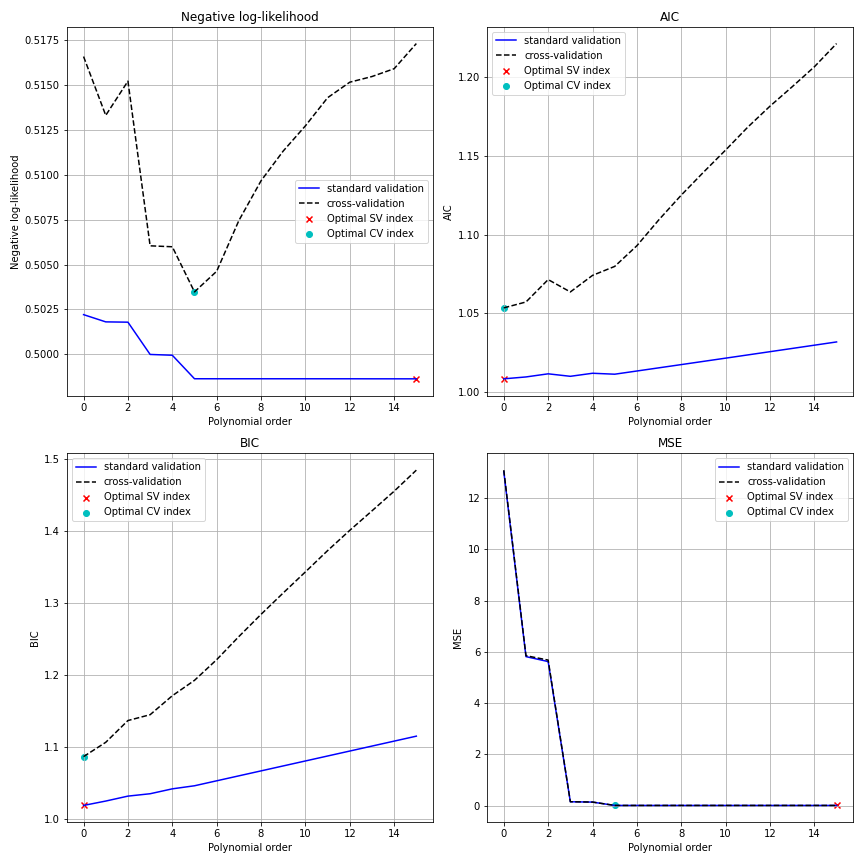
\includegraphics[width=\textwidth]{Q2b_fig2.png}
         \caption{$N_{samples} = 1000$, free variance.}
     \end{subfigure}
     \hfill
     \begin{subfigure}[b]{0.45\textwidth}
         \centering
         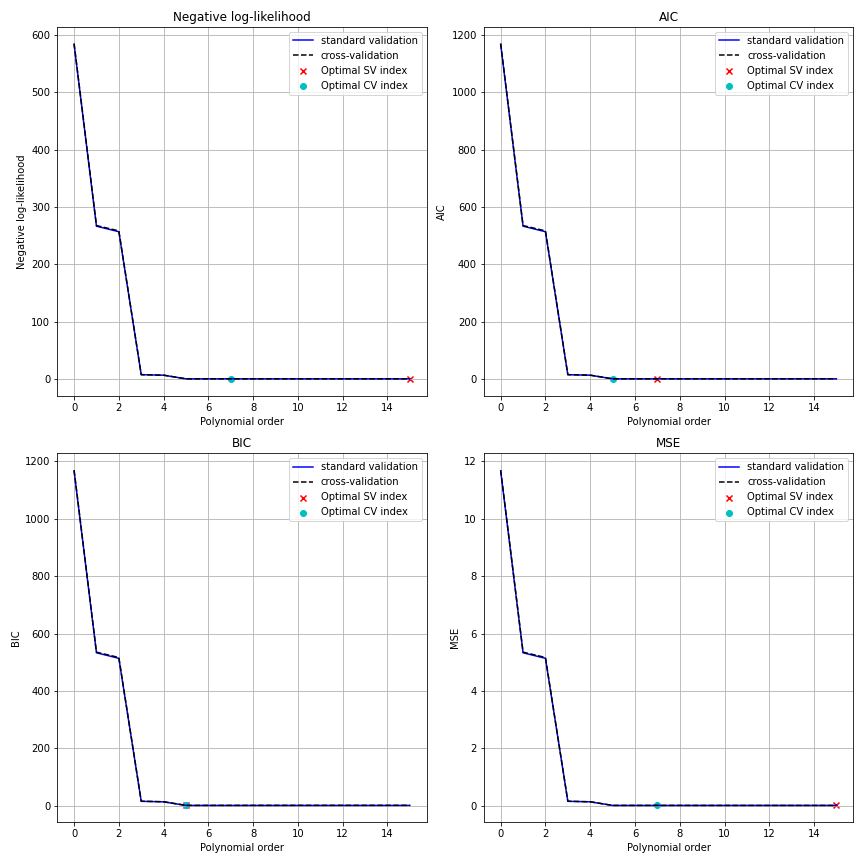
\includegraphics[width=\textwidth]{Q2b_fig2_1.png}
         \caption{$N_{samples} = 1000$, fixed variance.}
     \end{subfigure}
     
     \begin{subfigure}[b]{0.45\textwidth}
         \centering
         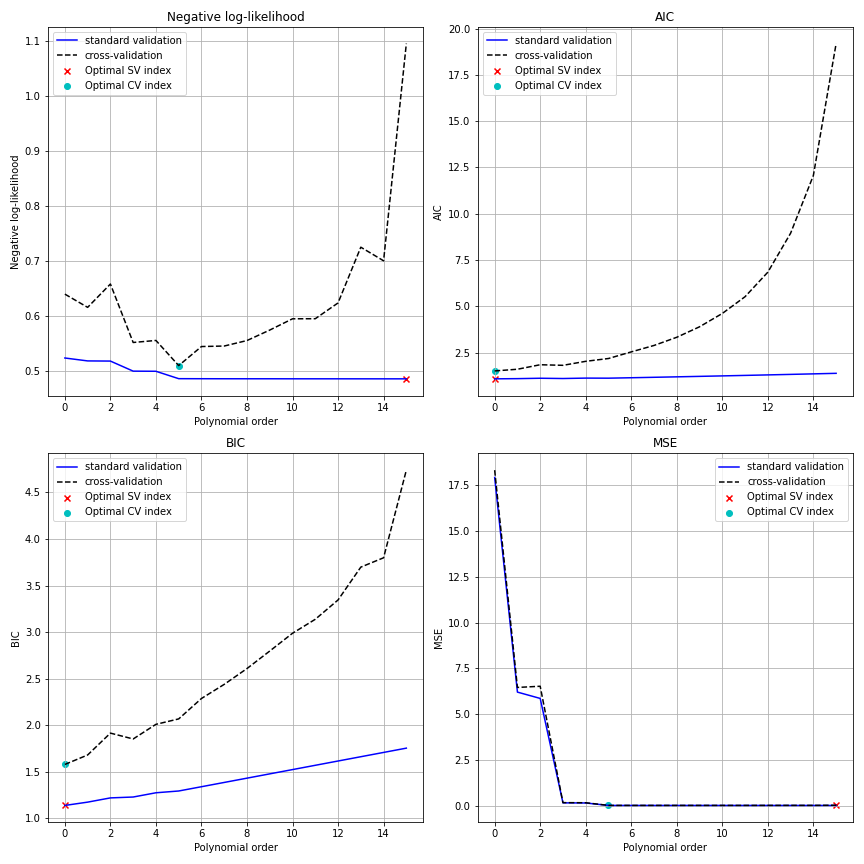
\includegraphics[width=\textwidth]{Q2b_fig2_2.png}
         \caption{$N_{samples} = 100$, free variance.}
     \end{subfigure}
     \hfill
     \begin{subfigure}[b]{0.45\textwidth}
         \centering
         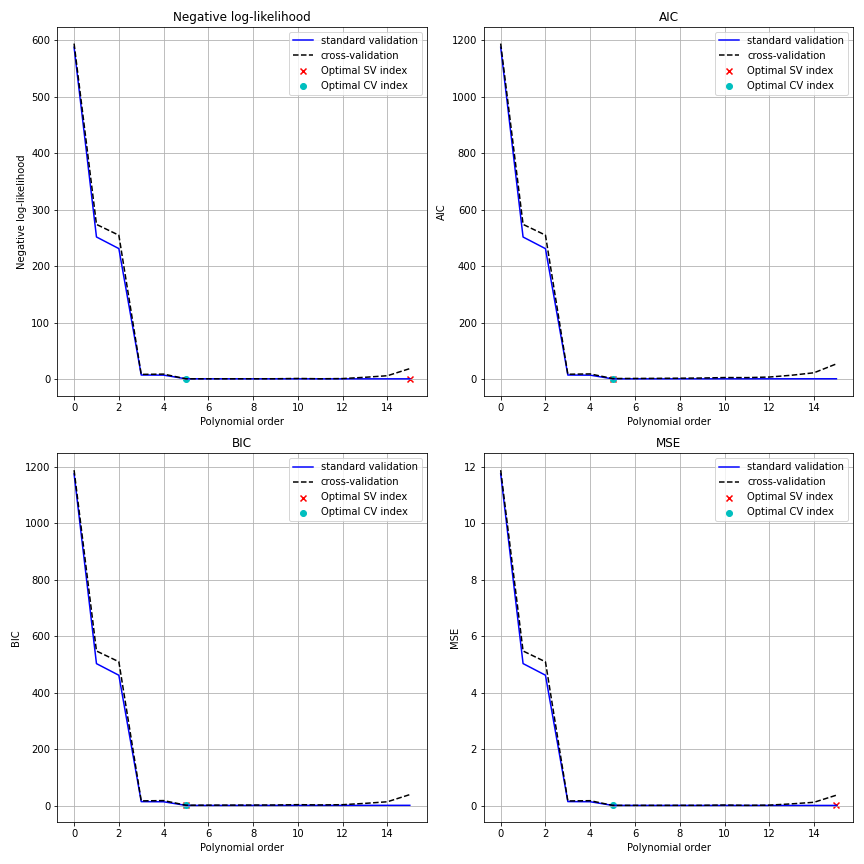
\includegraphics[width=\textwidth]{Q2b_fig2_3.png}
         \caption{$N_{samples} = 100$, fixed variance.}
     \end{subfigure}
        \caption{The results from the model selection investigation for four selection methods as a function of the model polynomial order. In a) 1000 samples were drawn from $f(x)$ and the model variance was found using maximum likelihood estimation. In b) 1000 samples were used and the model variance was set to $\sigma^2=0.1^2$. In c) 100 samples were used and the model variance was found using maximum likelihood estimation. In d) 100 samples were used and the model variance was set to $\sigma^2=0.1^2$.}
        \label{fig:Q2b_2}
\end{figure}

In Figure \ref{fig:Q2b_2} the results of this investigation are shown. In Figure \ref{fig:Q2b_2}a) 1000 samples were drawn and the model variance $\hat{\sigma}$ was left as a free parameter. In Figure \ref{fig:Q2b_2}b) the same number of samples was used but the model variance was set to the true model variance $\hat{\sigma}=\sigma=0.1$. In Figures \ref{fig:Q2b_2}c) and d) the same variance investigation difference is present, but the number of samples was reduced to 100.

If Figure \ref{fig:Q2b_2}a), it is clear that the NLL and the MSE metrics exhibit similar responses for the standard and cross-validation setting. In the standard setting, the optimal models are the ones with the highest model order. In the cross-validation setting, the optimal models are those of order five. However, both the AIC and BIC metrics select the smallest model order. This indicates that the NLL of the model at different orders is not as significant as the number of model parameters. To investigate why this is the case, the model variance was set to constant. The rationale behind this decision is because the variance acts are a normalisation factor in the model log-likelihood, and thus it may be that the model fits poorly, but if $\hat{\sigma}$ is large then the log-likelihood will be small. Figure \ref{fig:Q2b_2}b) confirms this idea, as the four metrics return similar optimal model orders in the standard setting and the cross-validation setting. The AIC and BIC metrics perform better in the standard setting, as opposed to the NLL and MSE methods, which shows that the inclusion of the number of parameters benefits the model selection process. 

In Figure \ref{fig:Q2b_2}c) the number of samples was reduced, and it is clear that the NLL and MSE metrics select the optimal model order in the cross-validation setting, while the AIC and BIC choose the simplest model. For the NLL and MSE metrics, the standard setting may bias itself towards a higher model order, and the inclusion of k-fold cross-validation in this investigation clearly highlights the importance of not testing the model on the data used to optimise the model parameters. In Figure \ref{fig:Q2b_2}d),  the flexibility afforded to the model through the variance parameter was removed, and improved responses are seen in all four metrics. Interestingly, in the low sample setting, both the AIC and BIC metrics select a model order of five in both the standard and cross-validation settings. This may suggest that these metrics are favourable in settings where the number of samples is limited. 

\subsubsection{Bias-variance investigation}

Not only can we investigate the effect of the metrics, but we can also investigate the model bias over the $x$ domain of interest. To calculate the bias, we can perform Monte Carlo estimation of the expectation term. The bias is given as 
\begin{equation}
    \text{bias}(x) = f_{\omega_{opt}}(x) - \mathbb{E}\{ x^{0}\cdot\omega_0 + x^{1}\cdot\omega_1 + \cdots + x^{K}\cdot\omega_K\}.
\end{equation}
Furthermore, the variance of the model is given as 
\begin{equation}
\text{variance}(x) = \mathbb{E} \{ \left[\left( x^{0}\cdot\omega_0 + x^{1}\cdot\omega_1 + \cdots + x^{K}\cdot\omega_K\right) - \mathbb{E}\{ x^{0}\cdot\omega_0 + x^{1}\cdot\omega_1 + \cdots + x^{K}\cdot\omega_K\}\right]^2 \}.
\end{equation}

For this investigation, the results of the bias-variance Monte Carlo estimation process is given in Figure \ref{fig:Q2b_3}. Note that for this investigation, the model variance was a free parameter. In Figure \ref{fig:Q2b_3}a) the model variance of the different metrics is shown. It is clear that the NLL and MSE results are bear a large number of similarities, and the AIC and BIC results are very similar. The AIC and BIC bias is the same form as the data, which is a result of the optimal model order that was selected, which was often a zero-th order polynomial. Hence, the bias is merely a centered version of the data, as we model determines the constant offset term alone. The NLL and MSE bias appears to be the worst at the end conditions, and fluctuates at the sections in the data with sharpest gradient changes. 

In figure \ref{fig:Q2b_3}b) the variance is shown for the four metrics. The variance in the AIC and BIC metrics is constant as the optimal model order is zero, and thus the variance is simply a function of how the constant offset term is estimated. For the NLL and MSE metrics, there is a large variance at the right-most section of the data, which suggests that the models vary heavily as a function of the sampled data in this region. In figure \ref{fig:Q2b_3} the bias-variance ratio is shown and the result of normalising the bias indicates that the model varies strongly around the regions of strong gradient change in the data.

\begin{figure}[!htb]
     \centering
     \begin{subfigure}[b]{0.45\textwidth}
         \centering
         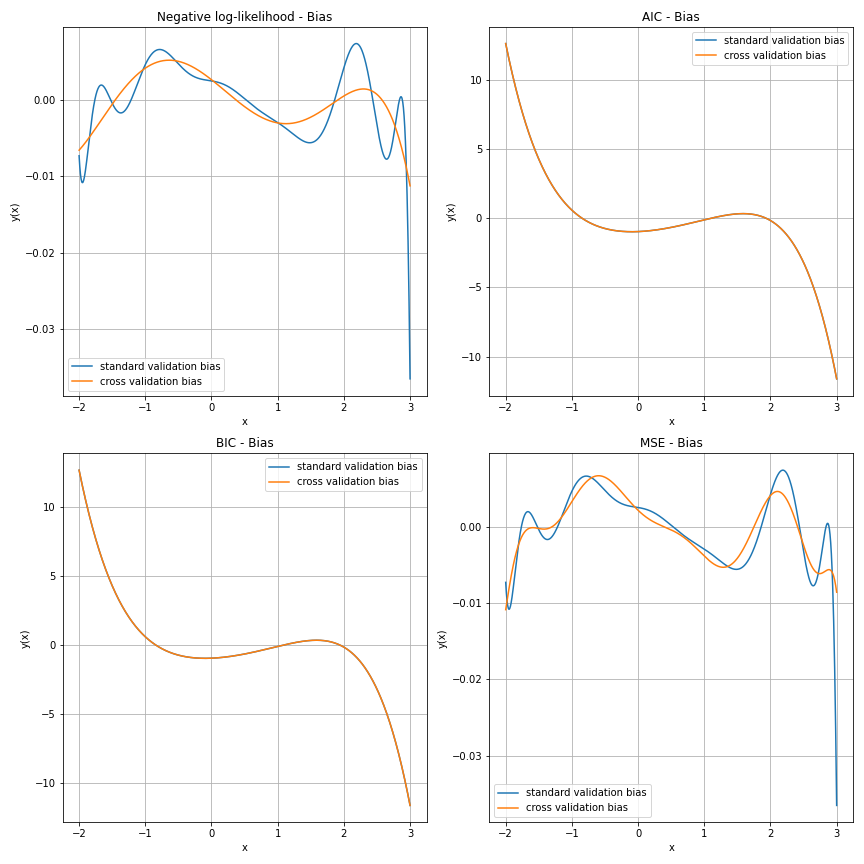
\includegraphics[width=\textwidth]{Q2b_fig3.png}
         \caption{Model bias.}
     \end{subfigure}
     \hfill
     \begin{subfigure}[b]{0.45\textwidth}
         \centering
         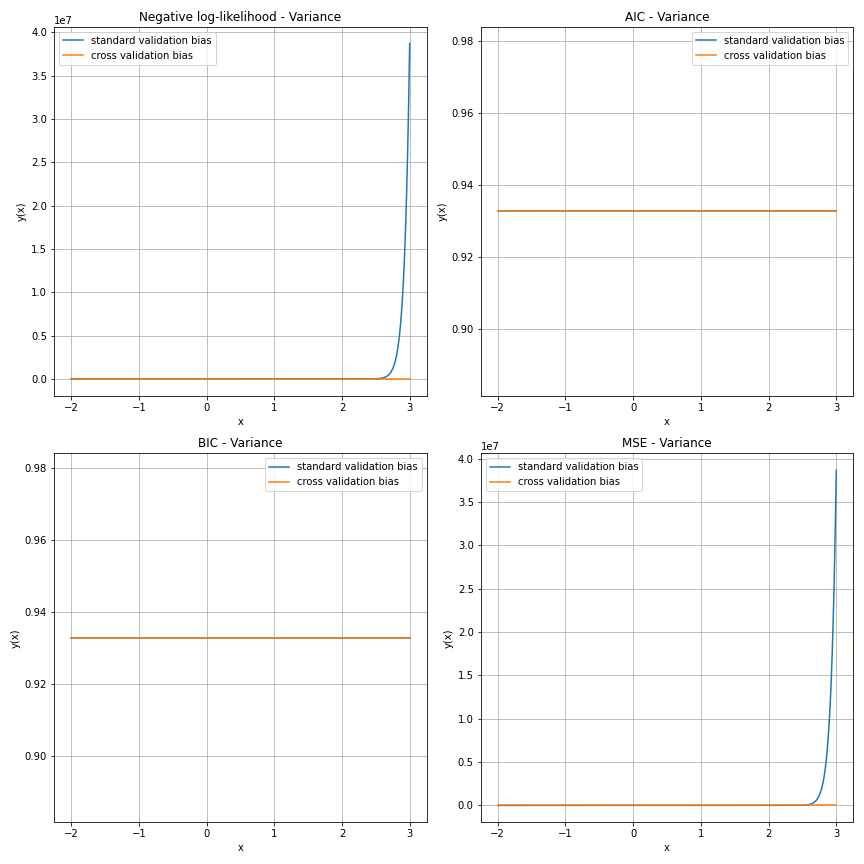
\includegraphics[width=\textwidth]{Q2b_fig4.png}
         \caption{Model variance.}
     \end{subfigure}
     
     \begin{subfigure}[b]{0.45\textwidth}
         \centering
         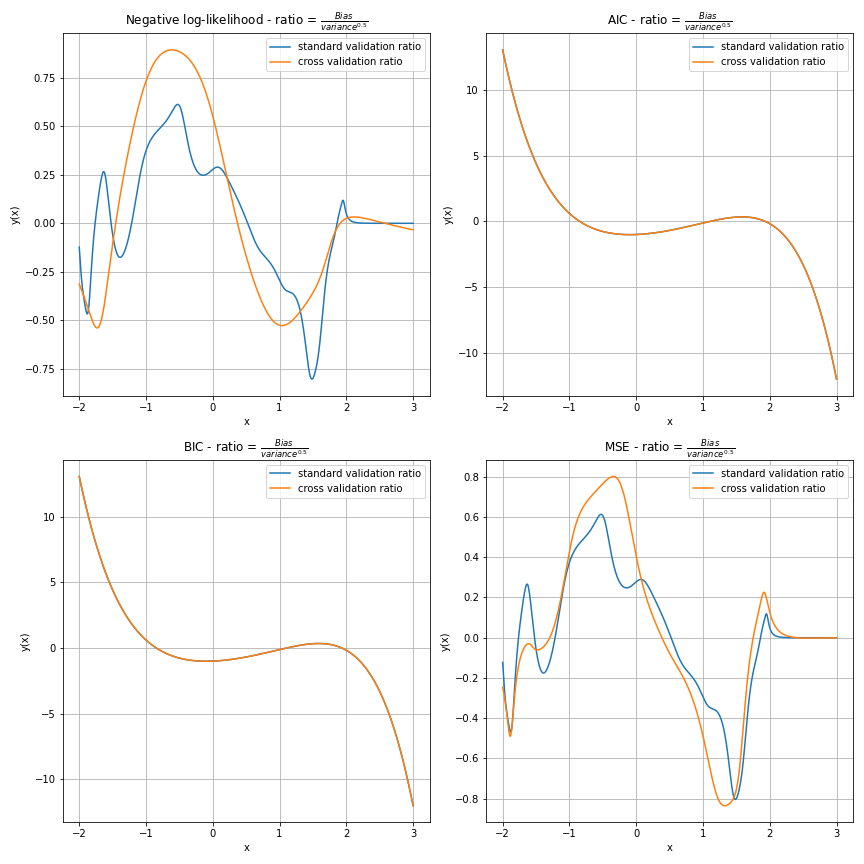
\includegraphics[width=\textwidth]{Q2b_fig5.png}
         \caption{bias-variance ratio.}
     \end{subfigure}
        \caption{The model bias and variance for the optimal polynomial order from the different model selection methods using model validation on all the training data and by performing k-fold cross validation. Note that in this example the model variance was a free parameter, and the AIC and BIC metrics selected the optimal order as zero. Hence the bias resembles the zero-centered data and the variance is constant.}
        \label{fig:Q2b_3}
\end{figure}

\clearpage

\section{Question 3}

Consider a model 
\begin{equation}
x(t_n;\theta_1, \theta_2) = \theta_1 \cdot \sin \left(2\cdot\pi\cdot t_n\right) + \epsilon_n(\theta_2),
\end{equation}
where $\theta_1$ is the amplitude of the sinusoid and $\theta_2$ is the scaling parameter of the zero-mean noise variable $\epsilon_n(\theta_2)$. The time signal is $0 \leq t \leq 10$ and the sampling frequency is approximately 100Hz.

\subsection{Model visualisation}

For $\theta_1 = 5$ and $\theta_2 = 1$, it is possible to investigate how different assumed noise distributions affect a generated signal. The three noise distributions of interest are \emph{i)} Gaussian noise, \emph{ii)} Laplacian noise, and \emph{iii)} Student-t noise with 1 degree of freedom. In Figure \ref{fig:Q3a_1} the generated signal is superimposed over the expected generated signal. The Laplacian and Student-t distributions have larger tails, and thus the noise in the generated signal appears to be stronger. If $\theta_2$ was to increase, we would expect the Gaussian distribution to be better constrained around the expected signal as its tails are less significant.
\begin{figure}[!htb]
    \centering
    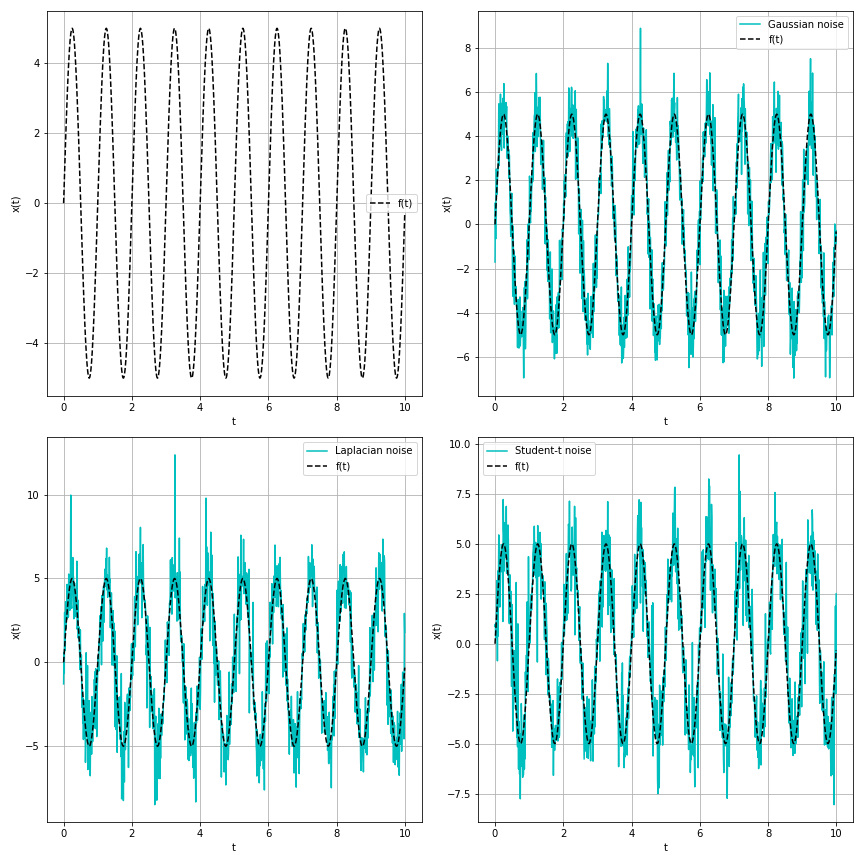
\includegraphics[scale = 0.4]{Q3a_fig1.png}
    \caption{The generated signals under different noise distributions.}
    \label{fig:Q3a_1}
\end{figure}

\subsection{Model estimation}

Under the assumed model form, we can estimate the parameters $\hat{\theta}_1$ and $\hat{\theta}_2$ given some data from the model. In Figure \ref{fig:Q3b_1}, the observed data used for parameter estimation is shown. Notice the significant outlier in the data in the time range $t \in [9, 10]$. For this investigation, a Gaussian noise model and a Laplacian noise model formulation will be presented and discussed. From this, the optimal model parameters for the different noise models will be presented and their maximum likelihood estimators for each model will be discussed.
\begin{figure}[!htb]
    \centering
    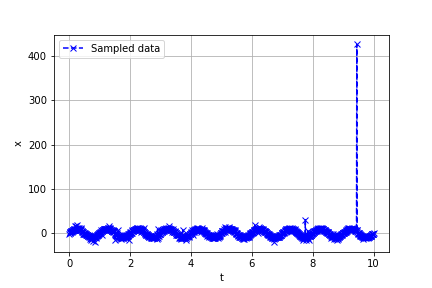
\includegraphics[scale = 0.7]{Q3b_fig1.png}
    \caption{The sampled data for the maximum likelihood estimation problem.}
    \label{fig:Q3b_1}
\end{figure}

\subsubsection{Gaussian noise problem formulation}
First, the Gaussian model formulation will be presented and discussed. Given a dataset $\mathcal{D} = \{ \mathbf{T}, \mathbf{x}\}$, where $\mathbf{T} = [t_1, \cdots, t_N]^T$ and $\mathbf{x} = [x_1, \cdots, x_N]^T$, $\mathbf{T} \in \mathbb{R}^{N \times 1}$, $\mathbf{x} \in \mathbb{R}^{N \times 1}$, we assume that the following model:
\begin{equation}
x_n = f(t_n; \theta_1) + \epsilon_n,
\end{equation}
where $\epsilon_n \sim \mathcal{N}(0, \theta_2)$. For the simplicity of notation, let $\boldsymbol\theta = \left[\theta_1, \theta_2\right]$ and let  $f(t_n; \theta_1)$ be
\begin{equation}
f(t; \theta_1) = \theta_1 \sin \left(2 \cdot \pi \cdot t \right).
\end{equation}
The resulting conditional distribution is
\begin{equation}
p(x \vert t, \boldsymbol\theta) = \mathcal{N}(x \vert f(t), \theta_2^2) = \frac{1}{\sqrt{2\pi\theta_2^2}} \exp\left( -\frac{1}{2\theta_2^2}\left[x_n - f(t_n;\theta_1) \right]^2\right).
\end{equation}

The log-likelihood function for the Gaussian noise model is
\begin{equation}
\begin{aligned}[b]
\log p(\mathbf{x} \vert \mathbf{T}) &= \sum_{n=1}^{N} \log  p(x_n \vert t_n) \\
\mathcal{L}(\boldsymbol\theta) &= \sum_{n=1}^{N} \left( -\frac{1}{2}\log \left( 2\pi \right) -\frac{1}{2}\log \left( \theta_2^2 \right) - \frac{1}{2\theta_2^2} \left[ x_n - f(t_n;\theta_1)\right] ^2 \right).
\end{aligned}
\end{equation}

Let us derive the estimators for this problem. For the $\theta_1$ parameter, we can analytically solve for a closed form solution through
\begin{equation}
\begin{aligned}[b]
0 &= \frac{d\mathcal{L}}{d\theta_1} \\
&= \frac{d\mathcal{L}}{df} \cdot \frac{df}{d\theta_1} \\
&= 0 - 0 -\frac{1}{2\theta_2^2} \sum_{n=1}^{N} \left[x_n - f(t_n)\right]\cdot \sin \left(2 \cdot \pi \cdot t_n \right) \\
\sum_{n=1}^{N} \theta_1 \sin \left(2 \cdot \pi \cdot t_n \right)\cdot \sin \left(2 \cdot \pi \cdot t_n \right) &=  \sum_{n=1}^{N} x_n \sin \left(2 \cdot \pi \cdot t_n \right) \\
\hat{\theta}_1 &= \frac{\sum_{n=1}^{N} x_n \sin \left(2 \cdot \pi \cdot t_n \right)}{\sum_{n=1}^{N} \sin \left(2 \cdot \pi \cdot t_n \right)\cdot \sin \left(2 \cdot \pi \cdot t_n \right)}.
\end{aligned}
\end{equation}

For the $\theta_2$ parameter, the closed form solution for the estimator is given as
\begin{equation}
\begin{aligned}[b]
0 &= \frac{d\mathcal{L}}{d\theta_2} \\
&= \sum_{n=1}^{N} \left( 0 -\frac{2\theta_2}{2\theta_2^2} -\frac{-2}{2\theta_2^3}\left[ x_n - f(t_n;\theta_1)\right]^2 \right) \\
&= \sum_{n=1}^{N} \left( 0 - \frac{1}{\theta_2} + \frac{1}{\theta_2^3}\left[ x_n - f(t_n;\theta_1)\right]^2  \right) \\
&= \frac{1}{\theta_2} \sum_{n=1}^{N} \left( - 1 + \frac{1}{\theta_2^2}\left[ x_n - f(t_n;\theta_1)\right]^2  \right) \\
N \theta_2^2 &= \sum_{n=1}^{N}\left[ x_n - f(t_n;\theta_1)\right]^2 \\
\hat{\theta}_2 &= \sqrt{\frac{1}{N}\sum_{n=1}^{N}\left[ x_n - f(t_n;\theta_1)\right]^2}.
\end{aligned}
\end{equation}

\subsubsection{Laplacian noise model formulation}

If the assumption is that the model noise is generated from a Laplace distribution, then we need to follow a procedure similar to the Gaussian model to determine $\boldsymbol\theta$. The Laplace distribution is given as
\begin{equation}\label{eq:laplace}
L(x \vert \mu, b) = \frac{1}{2b} \exp\left(-\frac{1}{b}\vert x - \mu \vert \right),
\end{equation}
and the logarithm of this is
\begin{equation}\label{eq:log_laplace}
\log L(x \vert \mu, b) = -\log(2b) -\frac{1}{b}\vert x - \mu \vert.
\end{equation}

To use the Laplacian noise distribution, we are required to implement a \texttt{Python} method that takes in the model parameters and returns the logarithm of the Laplacian likelihood for a given $t$ sample. Figure \ref{fig:Q3b_laplace} demonstrates that Equation \eqref{eq:laplace} and Equation \eqref{eq:log_laplace} are implemented correctly, as the implemented function has the same shape as a \texttt{scipy.stats} Laplacian function.
\begin{figure}[!htb]
     \centering
     \begin{subfigure}[b]{0.45\textwidth}
         \centering
         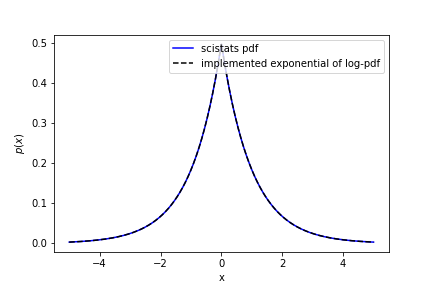
\includegraphics[width=\textwidth]{Q3b_fig4.png}
         \caption{Laplacian distribution.}
     \end{subfigure}
     \hfill
     \begin{subfigure}[b]{0.45\textwidth}
         \centering
         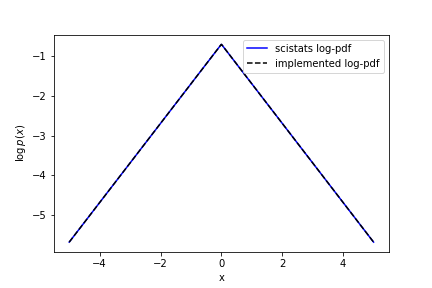
\includegraphics[width=\textwidth]{Q3b_fig3.png}
         \caption{Natural logarithm of Laplacian distribution.}
     \end{subfigure}
        \caption{A \texttt{Python} implementation of the Laplacian and log-Laplacian distribution. }
        \label{fig:Q3b_laplace}
\end{figure}

The next step in the Laplacian maximum likelihood formulation is to detail a process to solve for estimates of $\boldsymbol\theta$. Given a dataset $\mathcal{D} = \{ \mathbf{T}, \mathbf{x}\}$, where $\mathbf{T} = [t_1, \cdots, t_N]^T$ and $\mathbf{x} = [x_1, \cdots, x_N]^T$, $\mathbf{T} \in \mathbb{R}^{N \times 1}$, $\mathbf{x} \in \mathbb{R}^{N \times 1}$, we assume that the following model 
\begin{equation}
x_n = f(t_n; \theta_1) + \epsilon_n,
\end{equation}
where $\epsilon_n \sim L(0, \theta_2)$ is a Laplacian noise distribution and $\boldsymbol\theta = \left[\theta_1, \theta_2\right]$. The deterministic component of the model $f(t_n; \theta_1)$ is
\begin{equation}
f(t; \theta_1) = \theta_1 \sin \left(2 \cdot \pi \cdot t \right).
\end{equation}

The resulting conditional distribution is
\begin{equation}
p(x \vert t, \boldsymbol\theta) = L(x \vert f(t), \theta_2) = \frac{1}{2\theta_2} \exp\left( -\frac{1}{2\theta_2}\vert x_n - f(t_n;\theta_1) \vert \right),
\end{equation}
and the expected log-likelihood function we wish to maximise is
\begin{equation}
\begin{aligned}[b]
\log p(\mathbf{x} \vert \mathbf{T}) &= \sum_{n=1}^{N} \log p(x_n \vert t_n) \\
\mathcal{L}(\boldsymbol\theta) &= \sum_{n=1}^{N} \left( -\log(2\theta_2) -\frac{1}{\theta_2}\vert x - f(t_n;\theta_1) \vert \right). \\
\end{aligned}
\end{equation}
Now that we have formally presented the model, we can detail a methodology to determine the estimators of the model. To initialise this process, let us determine an estimator for $\theta_1$. The first step here is to derive the log-likelihood function with respect to $\theta_1$
\begin{equation}
\begin{aligned}[b]
0 &= \frac{d\mathcal{L}}{d\theta_1} \\
&= \frac{d\mathcal{L}}{df} \cdot \frac{df}{d\theta_1}. \\
\end{aligned}
\end{equation}

The complexity of this derivative comes from the absolute value over $\vert x - f \vert$. The derivative of an absolute value of an arbitrary function $f(x)$ is (let $u = f(x)$):
$\frac{d}{dx} \vert f(x) \vert = \frac{d}{du} \vert u \vert  \cdot \frac{du}{dx} = \frac{u}{\vert u \vert} \cdot \frac{du}{dx} = \frac{f(x)}{\vert f(x) \vert} \frac{df}{dx} = \text{sgn}(f(x)) \frac{df}{dx}$

Thus, let $u = x_n - f(t_n; \theta_1)$:
\begin{equation}
\begin{aligned}[b]
0 &=- \frac{1}{\theta_2}\sum_{n=1}^{N} \frac{d}{du} \vert u \vert  \cdot \frac{du}{d\theta_1}  \\
&= - \frac{1}{\theta_2}\sum_{n=1}^{N} \frac{u}{\vert u \vert}   \cdot \frac{du}{d\theta_1} \\
&= - \frac{1}{\theta_2}\sum_{n=1}^{N} \frac{x_n - f(t_n; \theta_1)}{\vert x_n - f(t_n; \theta_1) \vert}   \cdot -\sin \left(2 \cdot \pi \cdot t_n \right) \\
&= \frac{1}{\theta_2}\sum_{n=1}^{N} \frac{\sin \left(2 \cdot \pi \cdot t_n \right)\left(x_n - \theta_1 \sin \left(2 \cdot \pi \cdot t_n \right) \right)}{\vert x_n - \theta_1 \sin \left(2 \cdot \pi \cdot t_n \right) \vert} \\
\theta_1 \sum_{n=1}^{N}\frac{\sin \left(2 \cdot \pi \cdot t_n \right)\left( \sin \left(2 \cdot \pi \cdot t_n \right) \right) }{\vert x_n - \theta_1 \sin \left(2 \cdot \pi \cdot t_n \right) \vert} &= \sum_{n=1}^{N}\frac{\sin \left(2 \cdot \pi \cdot t_n \right)\left(x_n \right)}{\vert x_n - \theta_1 \sin \left(2 \cdot \pi \cdot t_n \right) \vert}.\\
\end{aligned}
\end{equation}
It is clear that there is no analytical solution here as $\theta_1$ cannot be isolated. Thus, there is no closed-form solution to obtain the maximum likelihood estimate for the model with Laplacian noise. Thus, we will turn to numerical optimisation methods. A exhaustive grid search is also a potential log-likelihood function maximisation methodology, but  for this work numerical optimisation methods are preferred for computational simplicity. The \texttt{scipy.optimize.minimize} method will be used to determine the optimal model parameters

\subsubsection{Estimator comparison}
Now that formal methodologies have been presented to determine the model parameters for a Gaussian and Laplacian model, we can discuss how the optimal parameter affect the different models. In Table \ref{tab:Q3b_table1} the estimates for $\hat{\boldsymbol\theta}$ are shown the two noise types alongside the model log-likelihood for the observed data. 
\begin{table}[!htb]
\centering
\caption{The $\theta_1$ and $\theta_2$ parameters for the models with a Gaussian and Laplacian noise distribution assumption.}
\label{tab:Q3b_table1}
\begin{tabular}{@{}cccc@{}}
\toprule
Noise type & $\hat{\theta}_1$ & $\hat{\theta}_2$ & Data log-likelihood \\ \midrule
Gaussian & 10.324624 & 13.625959 & 4030.915 \\
Laplacian & 9.980851 & 1.791687 & 2276.378 \\ \bottomrule
\end{tabular}
\end{table}

As shown in Table \ref{tab:Q3b_table1}, the estimate $\hat{\theta}_1$ is similar for the different models. However, the estimate $\hat{\theta_2}$ is vastly different. Although the two parameters do not have the same effect in the noise distributions, we can use the variance of the models to compare the difference. For a Gaussian model the variance is $\text{var}_{Gauss}(x) = \hat{\theta}^2_1 = 185.78$ and for a Laplacian distribution the variance is $\text{var}_{Laplacian}(x) = 2\cdot\hat{\theta}_1^2 = 6.42$. Thus, it is clear to see that the variance in the Gaussian model is more than 20 times the Laplacian variance. The reason for this is the sensitivity of the Gaussian model to outliers. The outlier in the $t \in [9, 10]$ range has a severe effect on the Gaussian model parameters as the variance is a function of the squared sample error $e_n = (x_n - f(x_n))^2$, and thus the variance is skewed by this term.
\begin{figure}[!htb]
     \centering
     \begin{subfigure}[b]{0.49\textwidth}
         \centering
         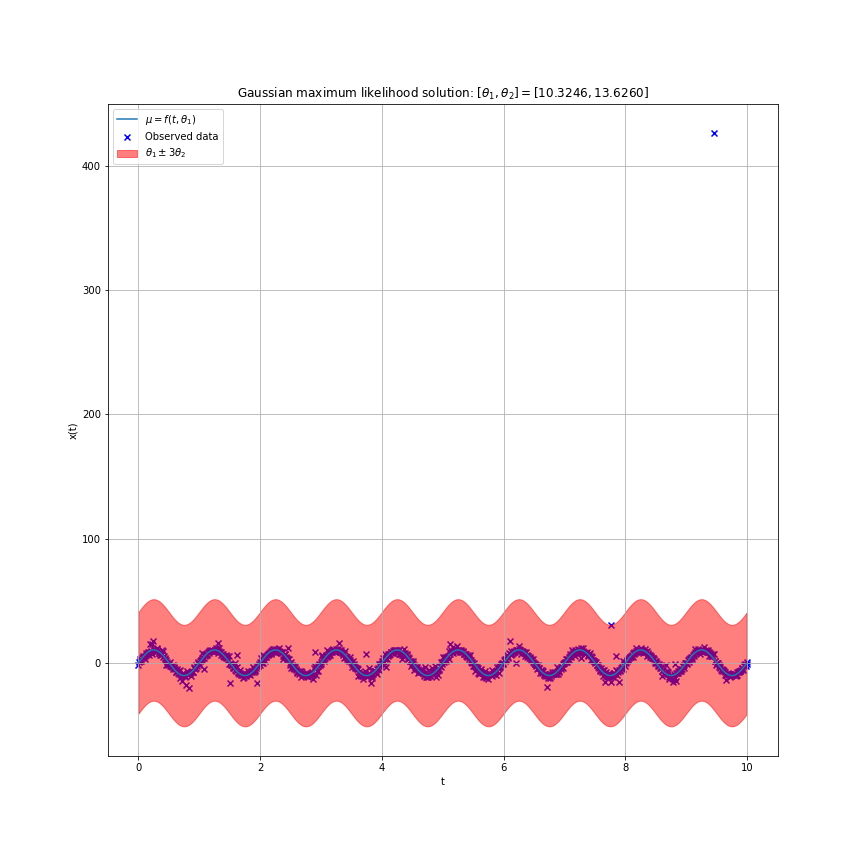
\includegraphics[width=\textwidth]{Q3b_fig5.png}
         \caption{Gaussian noise model.}
     \end{subfigure}
     \hfill
     \begin{subfigure}[b]{0.49\textwidth}
         \centering
         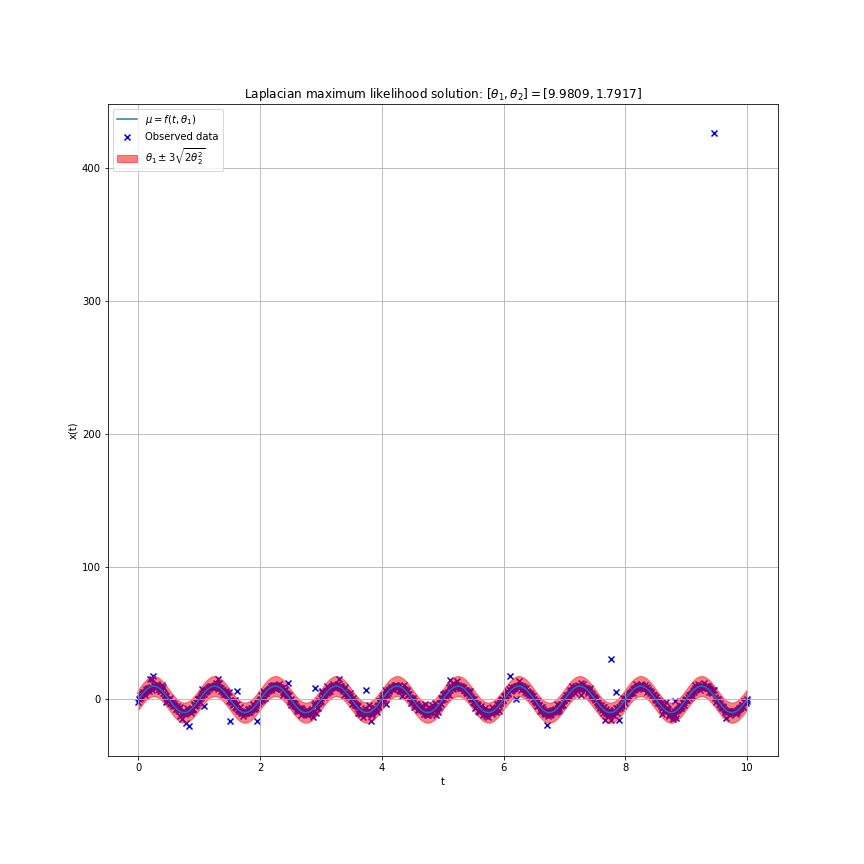
\includegraphics[width=\textwidth]{Q3b_fig6.png}
         \caption{Laplacian noise model.}
     \end{subfigure}
     
     \begin{subfigure}[b]{0.8\textwidth}
         \centering
         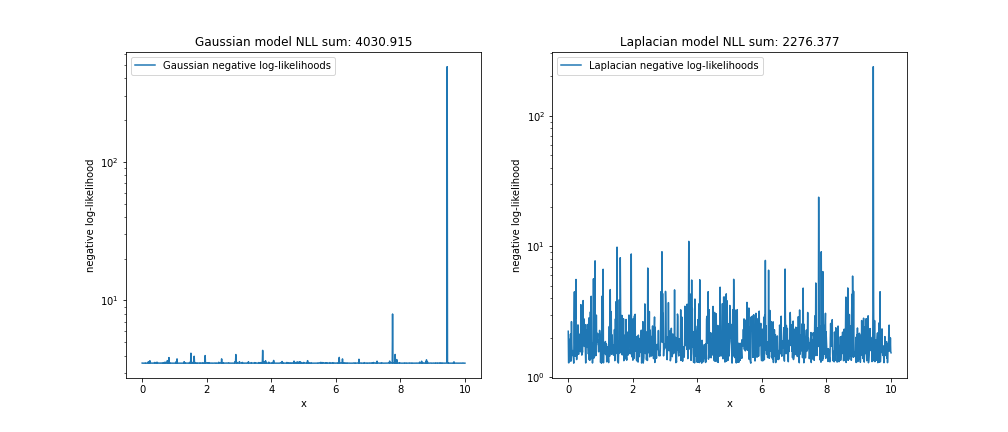
\includegraphics[width=\textwidth]{Q3b_fig8.png}
         \caption{Sample negative log-likelihood.}
     \end{subfigure}
        \caption{The optimal Gaussian and Laplacian models fitted to the sampled data in Figure \ref{fig:Q3b_1}. a) shows the the Gaussian model, b) shows the Laplacian model, and c) shows the sample negative log-likelihood for both models.}
        \label{fig:Q3b_2}
\end{figure}

In Figure \ref{fig:Q3b_2} the different models are visualised over the available observed data, and the observed data negative log-likelihood is shown. In Figures \ref{fig:Q3b_2}a) the large Gaussian variance is clear, whereas the Laplacian model variance, shown in Figure \ref{fig:Q3b_2}b), has a tighter bound over the $x$ parameter space as a function of time. In Figure \ref{fig:Q3b_2}c) the sample negative log-likelihood for the different models is shown, and the sensitivity to the outlier in the Gaussian model case is evident. For the Laplacian model, the outlier is still detectable, however its scale is far less significant than the Gaussian case.

\subsection{Model bias and variance}

Finally, it is also possible to investigate the choice of noise distribution for data generated from a Student t distribution with two degrees of freedom. Consider a model 
\begin{equation}
x(t_n;\boldsymbol\theta) = \theta_1 \cdot \sin \left(2\cdot\pi\cdot t_n\right) + \epsilon_n(\theta_2),
\end{equation}
where $\theta_1 = 5$ is the amplitude of the sinusoid and $\theta_2 = 1$ is the scaling parameter of the zero-mean Student t noise variable $\epsilon_n(\theta_2)$. The time signal is $0 \leq t \leq 10$ and the sampling frequency is 100Hz. In Figure \ref{fig:Q3c_1} data generated from the governing model is shown. The purpose of this investigation is to investigate a Gaussian and Laplacian model fit the available data. For this investigation, the model parameters are found using numerical optimisation techniques.
\begin{figure}[!htb]
    \centering
    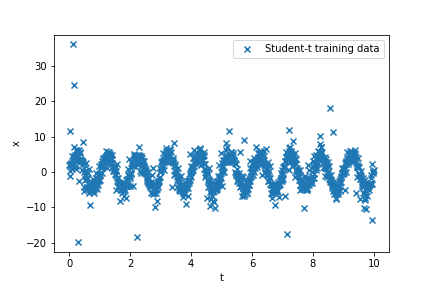
\includegraphics[scale=0.8]{Q3c_fig1.png}
    \caption{The data generated from $x_n=f(x_n)+\epsilon_n$, where the noise is sampled from a Student-t distribution with two degrees of freedom. The sampling frequency was $F_s=100Hz$.}
    \label{fig:Q3c_1}
\end{figure}

In Table \ref{tab:Q3b_table2}, the optimal model parameters for the Gaussian and Laplacian models is shown. In this case, both models recover the $\theta_1$ parameter within a tolerance of $1e^{-1}$. This tolerance may be coarse, but if the sampling frequency was increased it would be expected that this tolerance decrease. Additionally, the noise distribution variance is also similar. The Gaussian variance is $\text{var}_{Gauss}(x) = 7.271512$ and the Laplacian variance is $\text{var}_{Laplace}(x) = 7.580660$. This indicates that both models fit the data similarly. In Figure \ref{fig:Q3c_2}, the observed data is superimposed over the two models, and the sample negative log-likelihood is shown. The final metric we have available is to evaluate the data log-likelihood of the different models, and it is clear that the Gaussian model has a larger negative log-likelihood. This is attributed to the model sensitivity to outliers, and there are a number of clear outliers in the data due to the large tails of a Student t distribution.
\begin{table}[!htb]
\centering
\caption{The $\theta_1$ and $\theta_2$ parameters for the models with a Guassian and Laplacian noise distribution assumption.}
\label{tab:Q3b_table2}
\begin{tabular}{@{}cccc@{}}
\toprule
Noise type & $\hat{\theta}_1$ & $\hat{\theta}_2$ & Data log-likelihood \\ \midrule
Gaussian & 4.792795 & 2.696574 & 2410.921 \\
Laplacian & 4.994549 & 1.376650 & 2012.7520 \\ \bottomrule
\end{tabular}
\end{table}

\begin{figure}[!htb]
     \centering
     \begin{subfigure}[b]{0.49\textwidth}
         \centering
         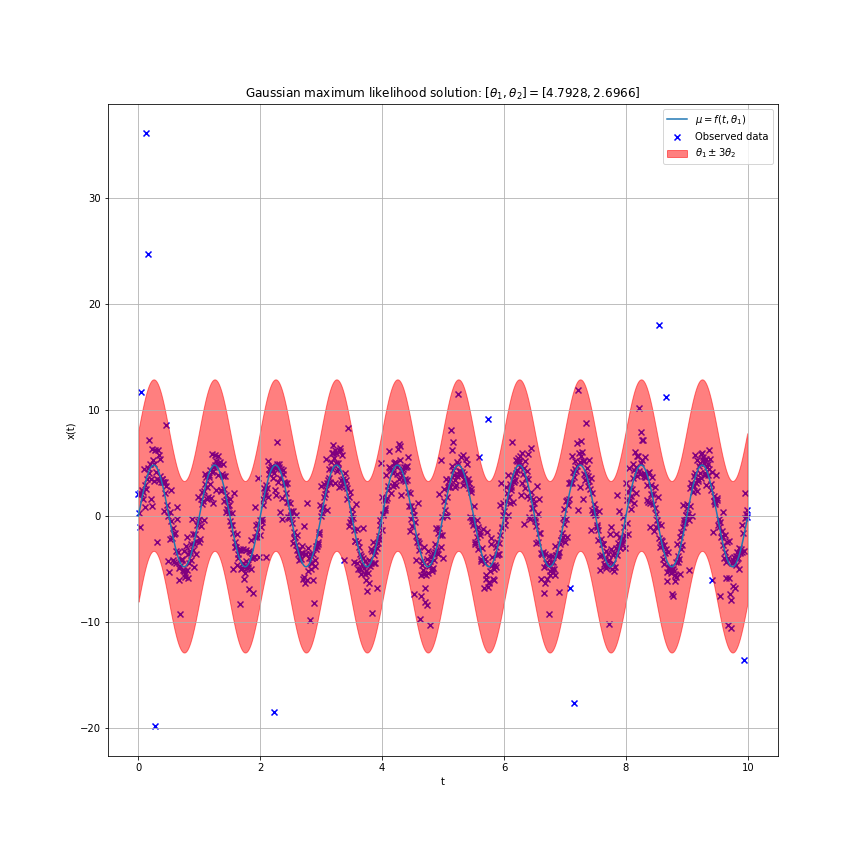
\includegraphics[width=\textwidth]{Q3c_fig2.png}
         \caption{Gaussian noise model.}
     \end{subfigure}
     \hfill
     \begin{subfigure}[b]{0.49\textwidth}
         \centering
         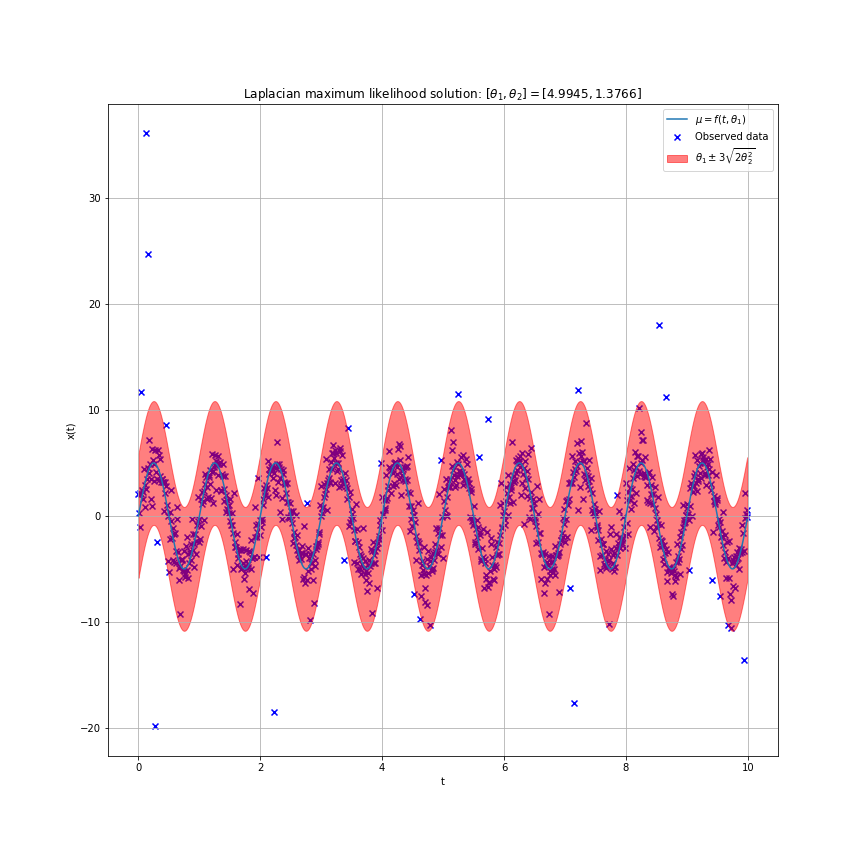
\includegraphics[width=\textwidth]{Q3c_fig3.png}
         \caption{Laplacian noise model.}
     \end{subfigure}
     
     \begin{subfigure}[b]{0.6\textwidth}
         \centering
         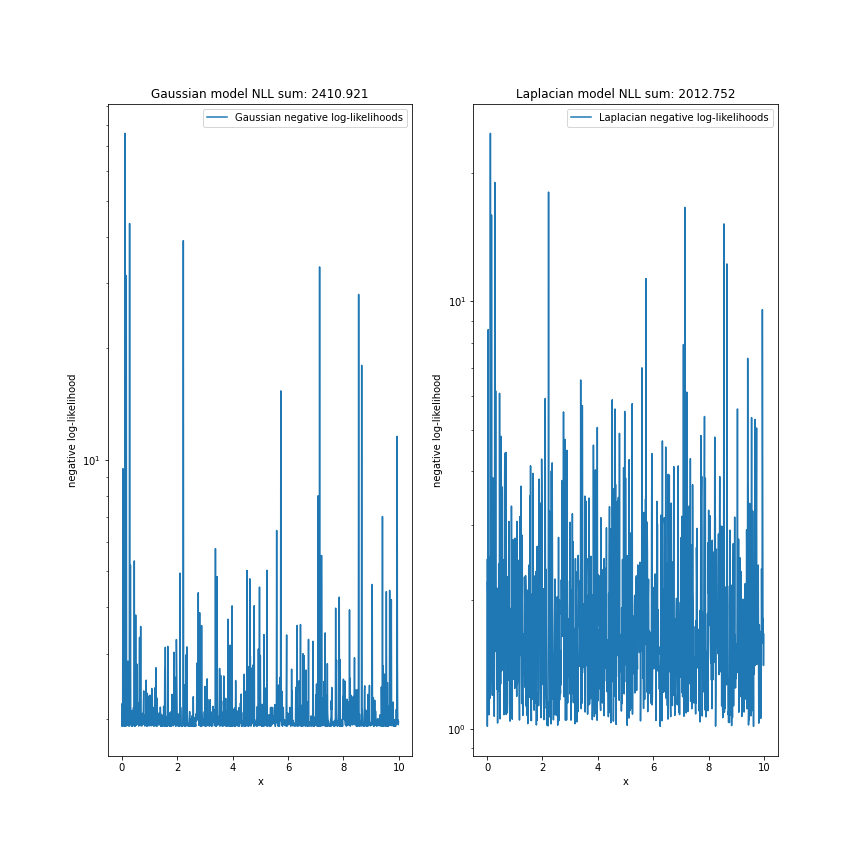
\includegraphics[width=\textwidth]{Q3c_fig5.png}
         \caption{Sample negative log-likelihood.}
     \end{subfigure}
        \caption{The optimal Gaussian and Laplacian models fitted to the sampled data in Figure \ref{fig:Q3c_1}. a) shows the the Gaussian model, b) shows the Laplacian model, and c) shows the sample negative log-likelihood for both models.}
        \label{fig:Q3c_2}
\end{figure}


Finally, we can also investigate how the estimate $\hat{\theta}_1$ varies for the different models as a function of the number of data samples. The number of samples is controlled by specifying the sampling frequency though $F_s = \frac{N_{samples}}{t_{end}}$, where $t_{end} = 10$. In Figure \ref{fig:Q3c_3}, the bias, variance an expected value of $\theta_1$ is shown. Figure \ref{fig:Q3c_3} clearly shows how the bias and variance of the Gaussian estimators are equivalent as a function of the number of samples, and tend towards the same value as the number of samples increases. There is also a clear insufficient number of samples point, with a clear observable inflection point present in Figure \ref{fig:Q3c_3}.
\begin{figure}[!htb]
    \centering
    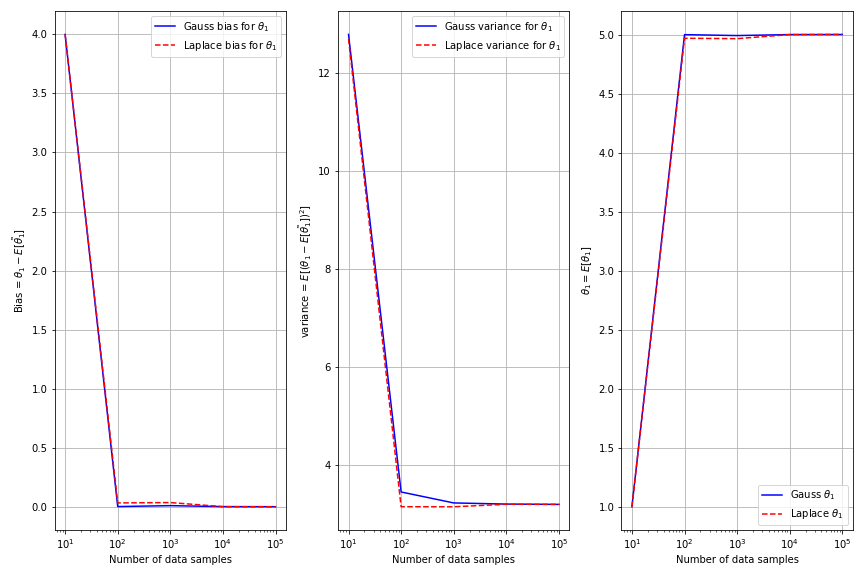
\includegraphics[scale = 0.5]{Q3c_fig6.png}
    \caption{The bias, variance and expected value for $\theta_1$ as a function of the number of data samples for the Gaussian and Laplacian noise models.}
    \label{fig:Q3c_3}
\end{figure}

\clearpage

\section{Question 4}

Consider a single-degree of freedom system with the following equation of motion:
\begin{equation}\label{eq:linear_system_eq}
m \cdot \ddot{x} + c \cdot \dot{x} + k \cdot x = f(t).
\end{equation}

where $m = 1$, $c = 10$ and $k = 1000$ for all investigations that follow. The sampling frequency $F_s$ is set to $F_s = 10e^3$ and the end time is $t_{end}=10$ seconds. The initial displacement and velocity of the system are $x_0 = 1e^{-3}$ and $\dot{x}_0 = -1.0$ respectively. The system of interest is a linear dynamical system where we know the second order differential equation of the system, and we can write as a first order differential equation through
\begin{equation}
\begin{aligned}[b]
\begin{bmatrix}
\dot{x} \\
\ddot{x}
\end{bmatrix} &= 
\begin{bmatrix}
0 & 1 \\
-\frac{k}{m} & -\frac{c}{m} \\
\end{bmatrix}
\begin{bmatrix}
x \\
\dot{x}
\end{bmatrix}+
\begin{bmatrix}
0 \\
\frac{f(t)}{m}
\end{bmatrix}, \\
&=
\begin{bmatrix}
0 & 1 \\
-\frac{k}{m} & -\frac{c}{m} \\
\end{bmatrix}
\begin{bmatrix}
x \\
\dot{x}
\end{bmatrix}+
\begin{bmatrix}
0 \\
\frac{1}{m}
\end{bmatrix}
\begin{bmatrix}
f(t)
\end{bmatrix}.
\end{aligned}
\end{equation}

In matrix-vector notation, this is given as
\begin{equation}
\dot{\mathbf{x}}(t) = \mathbf{A}\mathbf{x}(t) + \mathbf{B}\mathbf{u}(t)
\end{equation}

There are numerous methods available to solve of the ordinary differential equation (ODE) if we know the initial state $\mathbf{x}(0)$ of the system. The problem that we seek a solution to is the computation the integral
\begin{equation}
x(t) = \int_{\mathbf{x}(0)}^{t}\dot{\mathbf{x}}(\tau)d\tau.
\end{equation}

however it may be difficult to perform this integration analytically. In this case, we can use numerical integration techniques for ODEs. The simplest of these is Euler's method, which replaces the derivative $\dot{\mathbf{x}}(t)$ with the forward finite difference approximation $\dot{\mathbf{x}}(t) \approx \frac{\mathbf{x}(t + \Delta t) - \mathbf{x}(t)}{\Delta t}$, where $\Delta t$ is referred to as the step size. We can re-arrange to develop an approximation for $\mathbf{x}(t + \Delta t)$ through
\begin{equation}
\begin{aligned}[b]
\mathbf{x}(t + \Delta t) &\approx \mathbf{x}(t) + \Delta t \dot{\mathbf{x}}(t) \\
&\approx \mathbf{x}(t) + \Delta t  \left(  \mathbf{A}\mathbf{x}(t) + \mathbf{B}\mathbf{u}(t) \right) \\
&\approx \left( \Delta t \mathbf{A} + \mathbf{I} \right) \mathbf{x}(t) + \Delta t \mathbf{B}\mathbf{u}(t) \\
&\approx \mathbf{A}_d  \mathbf{x}(t) + \mathbf{B}_d \mathbf{u}(t), \\
\end{aligned}
\end{equation}

where
\begin{equation}
\mathbf{A}_d = \Delta t \mathbf{A} + \mathbf{I},
\end{equation}
and
\begin{equation}
\mathbf{B}_d = \Delta t \mathbf{B}.
\end{equation}

It is clear that we now have an approximation for the forward time state $\mathbf{x}(t + \Delta t)$, and we can use a recursive methodology to iteratively solve for $\mathbf{x}(t)$ on the interval $t \in \left[ 0, t_{end} \right]$, where $t_{end} >0$. The choice of the step size $\Delta t$ induces an error in referred to as the local truncation error, however information of this error is beyond the scope of this assignment. Interested readers can consult the works of Burden \cite{Burden2016} for more information. Thus, we can develop a discrete solution to the system using
\begin{equation}
\mathbf{x}(t_{k + 1}) = \mathbf{A}_d  \mathbf{x}(t_k) + \mathbf{B}_d \mathbf{u}(t_k),
\end{equation}
where $k \geq 0$ and $\mathbf{x}(0)$ must be given to initialise the solution. Naturally, Euler's method is one of many numerical integration techniques for ordinary differential equations, but alternative methods will not be discussed here. Interested readers can refer to \cite{Burden2016} for more information on numerical integration techniques for ODEs.

\subsection{Unforced system investigation}
For the first investigation, the forcing function $f(t)$ in Equation \eqref{eq:linear_system_eq} is equal to zero. The objective here is to determine how accurately one can recover the system matrix from an observed set of data. 

\subsubsection{System response}
 For the given model parameters, the displacement and velocity response as a function of time was determined using Euler ODE numerical integration. Figure \ref{fig:Q4a_1} shows the response on the system. Notice how the damping in the model reduces the response to zero, as it dissipates energy from the system.
\begin{figure}
    \centering
    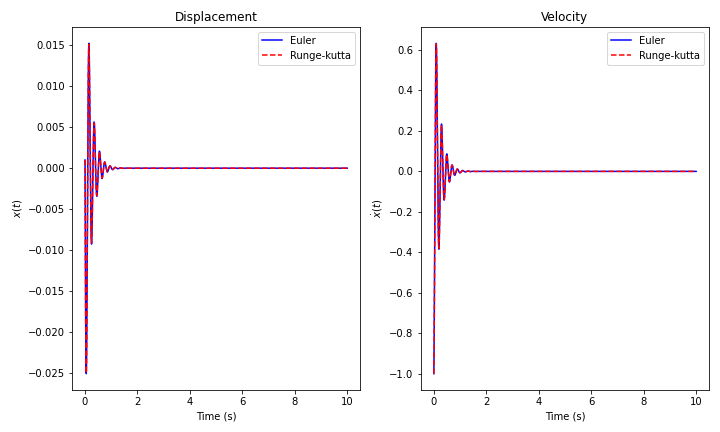
\includegraphics[scale = 0.5]{Q4a_fig1.png}
    \caption{The displacement and velocity response of the unforced system. The Euler and Runge-Kutta solutions are superimposed over one another to demonstrate that the sampling frequency $F_s$ is suitable.}
    \label{fig:Q4a_1}
\end{figure}

\subsubsection{System estimation}
To estimate the system parameters, the system matrix $\mathbf{A}$ can be estimated using
\begin{equation}
\hat{\mathbf{A}} = \left[ \left( \mathbf{X}_{n-1}^{T} \mathbf{X}_{n-1} \right) \mathbf{X}_{n-1}^{T} \mathbf{X}_{n} \right]^T,
\end{equation}
where $\mathbf{X}_{n-1}$ is given as
\begin{equation}
\mathbf{X}_{n-1} = 
\begin{bmatrix}
\mathbf{x}_0^T \\
\mathbf{x}_1^T  \\
\vdots \\
\mathbf{x}_{N-1}^T 
\end{bmatrix},
\end{equation}
and $\mathbf{X}_{n}$ is equal to
\begin{equation}
\mathbf{X}_{n} = 
\begin{bmatrix}
\mathbf{x}_1^T \\
\mathbf{x}_2^T  \\
\vdots \\
\mathbf{x}_{N}^T 
\end{bmatrix}.
\end{equation}

It is important to note here that the $n^{th}$ sample $\mathbf{x}_{n}$ consists of two terms $\mathbf{x}_{n} = \begin{bmatrix} x_{n} & \dot{x}_{n} \end{bmatrix}^T$. This is because we transformed the second order derivative into two first order derivatives. Thus, the $\mathbf{X}_{n}$ and $\mathbf{X}_{n-1}$ are matrices of size $\mathbb{R}^{\left(N-1\right) \times 2}$.

The recovered system matrix is
\begin{equation}
\hat{\mathbf{A}}_d = 
\begin{bmatrix}
1.00 &  1.00e^{-4} \\
-1.00e^{-1} &  9.99e^{-1} \\
\end{bmatrix},
\end{equation}
and the original system matrix is
\begin{equation}
\mathbf{A} = 
\begin{bmatrix}
1.00 &  1.00e^{-4} \\
-1.00e^{-1} & 9.99e^{-1} \\
\end{bmatrix}.
\end{equation}

Thus it is clear that we were able to recover the system matrix exactly. If we inspect the predicted model response in Figure \ref{fig:Q4a_2}, it is clear that we can predict the model response accurately under a variety of starting conditions. This accuracy occurs as the system parameters are constant through time, and thus the system matrix of the continuous system is constant. From Figures \ref{fig:Q4a_2}a) and b) it is clear that the predicted response and the numerically integrated response has minimal difference, with a maximum error tolerance of $1e^{-12}$.
\begin{figure}[!htb]
     \centering
     \begin{subfigure}[b]{0.49\textwidth}
         \centering
         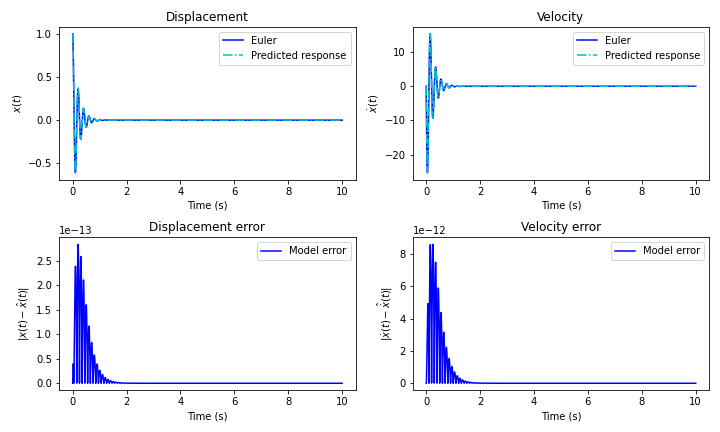
\includegraphics[width=\textwidth]{Q4a_fig2.png}
         \caption{$[x_0, \dot{x}_0] = [1, 0]$.}
     \end{subfigure}
     \hfill
     \begin{subfigure}[b]{0.49\textwidth}
         \centering
         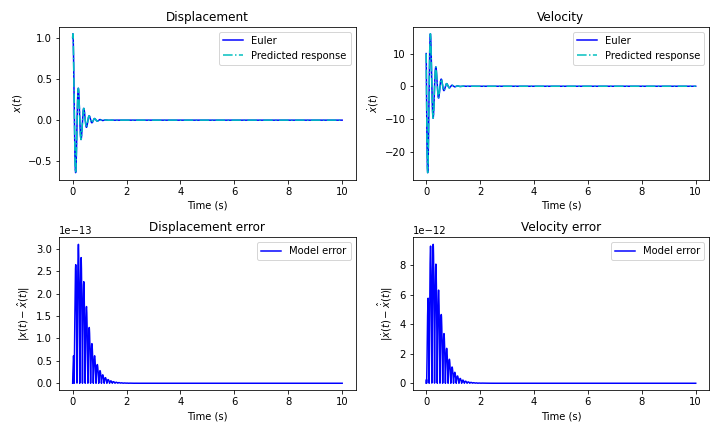
\includegraphics[width=\textwidth]{Q4a_fig2_1.png}
         \caption{$[x_0, \dot{x}_0] = [1, 10]$.}
     \end{subfigure}
        \caption{The predicted model displacement and velocity response and the absolute error between the actual and predicted model response under two different initial values. Notice that the predicted model is able to predict the response with great precision, regardless of the initial conditions. Note that the model noise $\sigma$ was assumed to be zero.}
        \label{fig:Q4a_2}
\end{figure}

\subsubsection{System parameter recovery}\label{section:unforced_parameter_recovery}

To recover the original parameters, we need some intrinsic knowledge of how the estimated system matrix is related to the true system matrix. If we assume that we know this relationship, for example (as was done in Q6.1.1 and Q6.1.2) if we know the governing physics of the problem (by using Newton's second law) to derive the ordinary differential equation (which contains the continuous system matrix), and by using finite differences to determine recursive equations used to find the discrete form of $\mathbf{x}(t)$ (which contains the discrete system matrix), then we at least have a reasonable starting point to try and recover these parameters. It is important to note that all of these components require a prior assumption regarding the physics of the data that we are modelling. If not, then there is definitely no way of doing so. 

If we assume that we know the relationship between the system matrix $\hat{\mathbf{A}}$ and the parameters of the model, then we can develop the following equation that relates the discrete-time system matrix $\hat{\mathbf{A}}_d$ to the continuous system matrix $\mathbf{A}_c$:
\begin{equation}
\begin{aligned}[b]
\hat{\mathbf{A}}_d = \Delta t \mathbf{A}_c + \mathbf{I} \\
\mathbf{A}_c = \frac{\hat{\mathbf{A}}_d - \mathbf{I}}{\Delta t}.
\end{aligned}
\end{equation}

From this, we can try to develop the final relationship between the model parameters (which are found in the continuous system matrix $\mathbf{A}$) using the fact that we have $d$ degrees of freedom:
\begin{equation}\label{eq:unforced_parameter_recovery}
\begin{aligned}[b]
\frac{\hat{\mathbf{A}}_d - \mathbf{I}}{\Delta t} =\mathbf{A}_c &= 
\begin{bmatrix}
\mathbf{0} & \mathbf{I} \\
-\mathbf{M}^{-1}\mathbf{K} & -\mathbf{M}^{-1}\mathbf{C} \\
\end{bmatrix} \\
\begin{bmatrix}
\mathbf{A}_{c, [1:dof, 1:2\cdot dof]} \\
\mathbf{A}_{c, [dof:2 \cdot dof, 1:2\cdot dof]}
\end{bmatrix}
&= \begin{bmatrix}
\mathbf{0} & \mathbf{I} \\
-\mathbf{M}^{-1}\mathbf{K} & -\mathbf{M}^{-1}\mathbf{C} \\
\end{bmatrix} \\
\begin{bmatrix}
\mathbf{A}_{c, [1:dof, 1:2\cdot dof]} \\
\mathbf{M} \mathbf{A}_{c, [dof:2 \cdot dof, 1:2\cdot dof]}
\end{bmatrix}
&= \begin{bmatrix}
\mathbf{0} & \mathbf{I} \\
-\mathbf{K} & -\mathbf{C} \\
\end{bmatrix}
\end{aligned}
\end{equation}

However, there is now a clear issue with the process as the left hand side of the second component $\mathbf{A}$ is a function of the system mass matrix $\mathbf{M}$. This complicates the solution as to recover any of the parameters we require knowledge of the masses of the system. Thus, I do not believe that one can recover all of the parameters, and you will need to have prior knowledge of one of the three components ($\mathbf{M}, \mathbf{C}, \mathbf{K}$) in order to be able to effectively solve for the other components.

If you do know one of the components, then we can decompose either the left or right hand size of Equation \eqref{eq:unforced_parameter_recovery} to solve for the other parameters.

\subsection{Forced system investigation}
For the second investigation, the forcing function $f(t)$ in Equation \eqref{eq:linear_system_eq} is equal to $f(t) = 100\cdot \cos \left( 2\cdot \pi \cdot t \right)$. The objective here is to determine how accurately one can recover the system matrix from an observed set of data when the system input is a function of time. 

\subsubsection{System response}
For the given model parameters, the displacement and velocity response as a function of time was determined using Euler ODE numerical integration. Figure \ref{fig:Q4b_1} shows the response on the system. Notice the system initially has some transient dynamics present within the first second, but after some time the response resembles a sinusoidal component. 
\begin{figure}
    \centering
    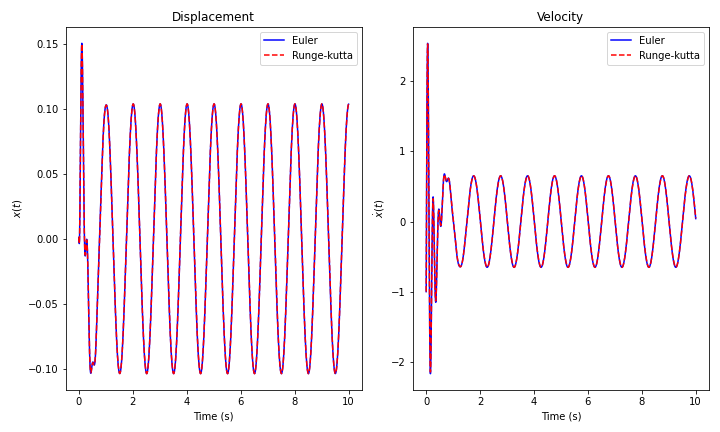
\includegraphics[scale = 0.5]{Q4b_fig1.png}
    \caption{The displacement and velocity response of the forced system. The Euler and Runge-Kutta solutions are superimposed over one another to demonstrate that the sampling frequency $F_s$ is suitable.}
    \label{fig:Q4b_1}
\end{figure}

\subsubsection{System estimation}
To estimate the system parameters, the System matrix $\mathbf{C}$ can be estimated using
\begin{equation}
\hat{\mathbf{C}} = \begin{bmatrix}\hat{A}_d & \hat{B}_d\end{bmatrix} = \left[ \left( \mathbf{S}_{n-1}^{T} \mathbf{S}_{n-1} \right) \mathbf{S}_{n-1}^{T} \mathbf{X}_{n} \right]^T,
\end{equation}
where $\mathbf{S}_{n-1}$ is given as
\begin{equation}
\mathbf{S}_{n-1} = 
\begin{bmatrix}
\mathbf{x}_0^T & \mathbf{u}_0^T \\
\mathbf{x}_1^T  & \mathbf{u}_1^T \\
\vdots \\
\mathbf{x}_{N-1}^T & \mathbf{u}_{N-1}^T
\end{bmatrix},
\end{equation}
$\mathbf{S}_{n}$ is given as
\begin{equation}
\mathbf{S}_{n} = 
\begin{bmatrix}
\mathbf{x}_1^T & \mathbf{u}_1^T \\
\mathbf{x}_2^T & \mathbf{u}_2^T  \\
\vdots \\
\mathbf{x}_{N}^T  & \mathbf{u}_N^T
\end{bmatrix},
\end{equation}
and $\mathbf{X}_{n}$ is equal to
\begin{equation}
\mathbf{X}_{n} = 
\begin{bmatrix}
\mathbf{x}_1^T \\
\mathbf{x}_2^T  \\
\vdots \\
\mathbf{x}_{N}^T 
\end{bmatrix}.
\end{equation}
It is important to note here that the $n^{th}$ sample $\mathbf{s}_{n}$ consists of three terms $\mathbf{x}_{n} = \begin{bmatrix} x_{n} & \dot{x}_{n} & u_n \end{bmatrix}^T$. Thus, the $\mathbf{S}_{n}$ and $\mathbf{S}_{n-1}$ are matrices of size $\mathbb{R}^{\left(N-1\right) \times 3}$ and $\mathbf{X}_{n}$ is of size $\mathbb{R}^{\left(N-1\right) \times 2}$.

The recovered system matrix is
\begin{equation}
\hat{\mathbf{C}} = 
\begin{bmatrix}
1 & 1e^{-4} & 0 \\
-1e^{-1} & 9.990075e^{-1} & 1.00005e^{-4} \\
\end{bmatrix},
\end{equation}

and the actual system matrix is
\begin{equation}
\mathbf{C} = 
\begin{bmatrix}
1 & 1e^{-4} & 0 \\
-1e^{-1} & 9.99e^{-1} & 1e^{-4} \\
\end{bmatrix}.
\end{equation}

Thus, we are able to recover the system matrix well. If we inspect the predicted model response in Figure \ref{fig:Q4b_2}, we see that the predicted model response for different initial conditions can be accurately determined by the model. The displacement and velocity errors under different starting conditions has a larger error than the unforced responses seen in Figure \ref{fig:Q4a_2}, however, the tolerance is still acceptable.
\begin{figure}[!htb]
     \centering
     \begin{subfigure}[b]{0.49\textwidth}
         \centering
         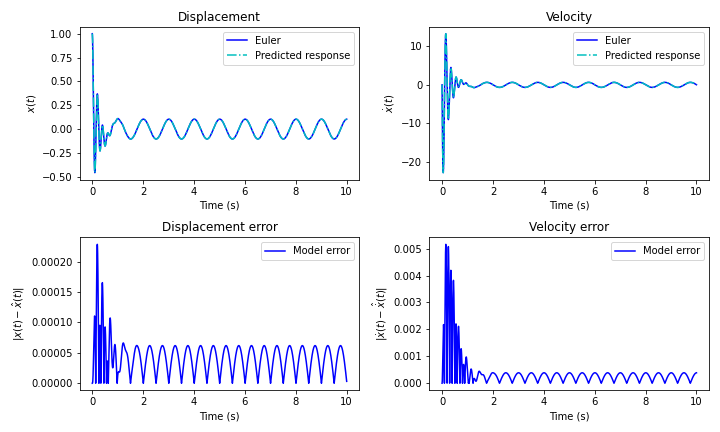
\includegraphics[width=\textwidth]{Q4b_fig2.png}
         \caption{$[x_0, \dot{x}_0] = [1, 0]$.}
     \end{subfigure}
     \hfill
     \begin{subfigure}[b]{0.49\textwidth}
         \centering
         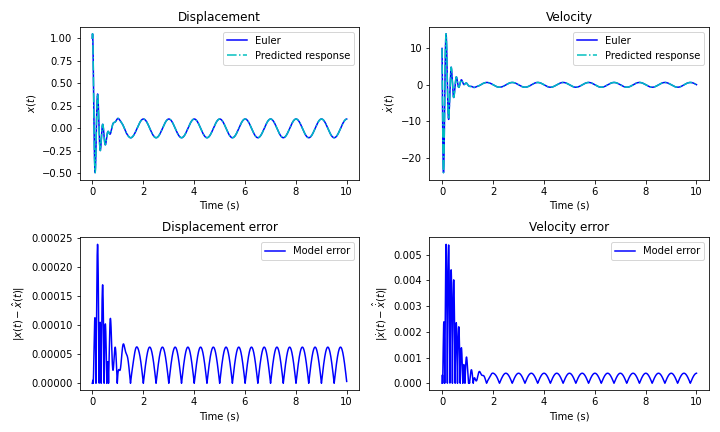
\includegraphics[width=\textwidth]{Q4b_fig2_1.png}
         \caption{$[x_0, \dot{x}_0] = [1, 10]$.}
     \end{subfigure}
        \caption{The predicted model displacement and velocity response and the absolute error between the actual and predicted model response under two different initial values. Notice that the predicted model is able to predict the response with great precision, regardless of the initial conditions. Note that the model noise $\sigma$ was assumed to be zero.}
        \label{fig:Q4b_2}
\end{figure}

\subsubsection{System parameter recovery}\label{section:forced_parameter_recovery}

In this forced system case, it is possible to recover the original system parameters. This is possible as the form of $\mathbf{B}_d$ allows us to recover the mass matrix exactly. If we assume that we know the governing physics of the system and the relationship between the continuous system matrices $\mathbf{A}$ and $\mathbf{B}$, and the discrete system matrix $\hat{\mathbf{C}} = \left[ \mathbf{A}_d, \mathbf{B}_d \right]$, we obtain
\begin{equation}
\begin{aligned}[b]
\mathbf{C} &= 
\begin{bmatrix} 
\mathbf{A}_d, & \mathbf{B}_d \\
\end{bmatrix} \\
&= 
\begin{bmatrix} 
\Delta t \mathbf{A} + \mathbf{I}, & \Delta t \mathbf{B} \\
\end{bmatrix} \\
&= 
\begin{bmatrix} 
\Delta t \mathbf{M}^{-1}
\begin{bmatrix}
\mathbf{0} & \mathbf{M} \\
-\mathbf{K} & -\mathbf{C} \\
\end{bmatrix} + \mathbf{I}, & \Delta t \begin{bmatrix} \mathbf{0} \\ \mathbf{M}^{-1} \end{bmatrix} \\
\end{bmatrix}.
\end{aligned}
\end{equation}

Thus, we can decompose $\mathbf{C}$ to help us recover specific terms. Specifically, let us assume that there are $d$ degrees of freedom in the problem. If we adopt this notation, then the size of $\mathbf{C}$ is $\mathbb{R}^{\left( 2\cdot d \right) \times \left( 3 \cdot d \right)}$. Thus, we can decompose $\hat{\mathbf{C}}$ into
\begin{equation}
\hat{\mathbf{C}} = \begin{bmatrix} C_{[1:2d, 1:2d]} &  C_{[1:2d, 2d:3d]} \end{bmatrix}
= \begin{bmatrix} \mathbf{A}_d &  \mathbf{B}_d \end{bmatrix}. \\
\end{equation}

Then, to solve for the mass matrix $\mathbf{M}$, we simply take $C_{[d:2d, 2d:3d]}$, multiply by $\frac{1}{dt}$ and invert the result of this step to get $\mathbf{M}$. Then, we can use the part of $\hat{\mathbf{C}}$ that corresponds to $\mathbf{A}_d$ to solve for $\mathbf{C}$ and $\mathbf{K}$. Specifically, we obtain
\begin{equation} \label{eq:forced_parameter_recovery}
\left( \frac{\mathbf{A}_d - \mathbf{I}}{\Delta t} \right) = 
\begin{bmatrix}
\mathbf{0} & \mathbf{I} \\
-\mathbf{M}^{-1}\mathbf{K} & -\mathbf{M}^{-1}\mathbf{C} \\
\end{bmatrix}. \\
\end{equation}

If we further decompose the left hand side of Equation \eqref{eq:forced_parameter_recovery} using the process described for in Section \label{section:unforced_parameter_recovery}, we can obtain specific solutions for $\mathbf{C}$ and $\mathbf{K}$. In Table \ref{tab:Q4b_table1}, the recovered parameters are shown and it is clear that we can recover the system parameters.
\begin{table}[!htb]
\centering
\caption{The recovered system parameters for the forced system.}
\label{tab:Q4b_table1}
\begin{tabular}{@{}ccc@{}}
\toprule
Parameter name & Actual parameter & Recovered parameter \\ \midrule
Mass & 1 & 0.9999469 \\
Spring stiffness & 1000 & 1000.044292 \\
Damping coefficient & 10 & 9.924691 \\ \bottomrule
\end{tabular}
\end{table}

\subsection{Model errors}
Consider an actual model that is given by
\begin{equation}\label{eq:time_varying_model}
m \ddot{x} + c \dot{x} + k \cdot \left( 1 + \alpha \sin\left(2 \cdot \pi \cdot t \right) \right) \cdot x = 100 \cdot \cos \left( 2 \cdot \pi \cdot t \right),
\end{equation}

where $0 \leq \alpha \leq 1$. Assume that we do not know the governing equation and assume the model form
\begin{equation}\label{eq:constant_model_LDS}
m \ddot{x} + c \dot{x} + k \cdot x = 100 \cdot \cos \left( 2 \cdot \pi \cdot t \right).
\end{equation}
In the actual model form given in Equation \eqref{eq:time_varying_model}, the model stiffness is a function of time, while the assumed model given in Equation \eqref{eq:constant_model_LDS} assumes that the model parameters are constant through time. The impact of this assumption limitation is that the actual system matrix $\mathbf{C}$ is a function of time, but the recovered matrix will be constant. The purpose of this investigation is thus to investigate how the assumed model predictive ability degrades as $\alpha$ varies from 0 to 1.

In Figure \ref{fig:Q4c_1} the true and predicted model response as a function of $\alpha$ is shown. Notice how in Figure \ref{fig:Q4c_1}a) the predicted response is accurate as $\alpha = 0$, but for $\alpha = 0.5$ and $\alpha = 1$ the predicted response degrades and the model error increases, as shown in Figures \ref{fig:Q4c_1}b) and c) respectively.  In Figure \ref{fig:Q4c_1}d), the estimated model parameters, which are constant, are shown as a function of $\alpha$. The process to determine the parameters is detailed in Section \ref{section:forced_parameter_recovery}. It is clear that the all estimated parameters are functions of $\alpha$, which indicates that the model is insufficiently flexible to model the data of interest. The mass increases substantially, while the damping coefficient decreases and the stiffness non-linearly increases and decreases.  
\begin{figure}[!htb]
     \centering
     \begin{subfigure}[b]{0.49\textwidth}
         \centering
         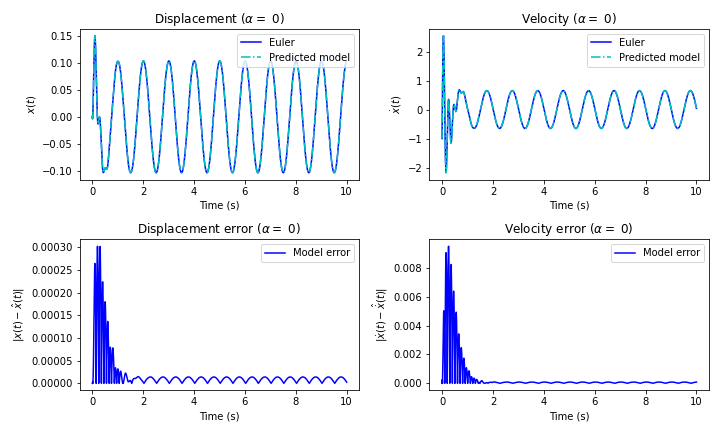
\includegraphics[width=\textwidth]{Q4c_fig2.png}
         \caption{$\alpha=0$ results.}
     \end{subfigure}
     \hfill
     \begin{subfigure}[b]{0.49\textwidth}
         \centering
         \includegraphics[width=\textwidth]{Q4c_fig4.png}
         \caption{$\alpha=0.5$ results.}
     \end{subfigure}
     
     \begin{subfigure}[b]{0.49\textwidth}
         \centering
         \includegraphics[width=\textwidth]{Q4c_fig6.png}
         \caption{$\alpha=1$ results.}
     \end{subfigure}
     \hfill
     \begin{subfigure}[b]{0.49\textwidth}
         \centering
         \includegraphics[width=\textwidth]{Q4c_fig7.png}
         \caption{System parameters.}
     \end{subfigure}
        \caption{The predicted model displacement, velocity response and the absolute error between the actual and predicted model response under the original initial conditions for $\alpha = 0, 0.5$ and $1$. Notice the degradation in the model response as $\alpha$ increases. In d) the estimated model parameters as a function of $\alpha$ are shown and it is clear that the predicted parameters are greatly affected by a stiffness that is a function of time.}
        \label{fig:Q4c_1}
\end{figure}

\section{Conclusion}
The purpose of this assignment is to introduce students to introductory topics of Engineering modelling. The covered concepts are in-depth and provided much insight into important aspects of modelling. I really enjoyed this assignment, as it made me think about the bias and variance of estimators, how one selects optimal model parameters and the sensitivity of the AIC and BIC metrics to the model variance, how the choice of noise distribution must be carefully selected for the observed data, and how to model dynamical systems in a probabilistic setting. These are just a few points that I enjoyed, and I believe that this assignment is a great introduction to the topics covered in the first block. 

\clearpage

%Print the bibliography
\printbibliography

\end{document}
